\documentclass[journal]{IEEEtran}

\usepackage[T1]{fontenc}
\usepackage[utf8]{inputenc}
\usepackage{lmodern}
\usepackage[spanish,es-noshorthands]{babel}
\addto\captionsspanish{\renewcommand{\tablename}{Tabla}}

\usepackage{amsmath}
\usepackage{graphicx}
\usepackage{color,array}
\usepackage{microtype}
\usepackage[colorlinks,urlcolor=blue,linkcolor=blue,citecolor=blue]{hyperref}

\usepackage{tabularx}
\usepackage{longtable}
\usepackage{booktabs}
\usepackage{tikz}
\usetikzlibrary{arrows.meta,positioning,fit,calc}

\raggedbottom
\sloppy
\tolerance=2000
\emergencystretch=5em
\hbadness=10000
\newcommand{\tablefont}{\small}

\begin{document}

\title{Generación de consultas SQL a partir de lenguaje natural aplicado al ERP Fail Fast
}

\author{Beatriz Natalia Serrano, Martín Santos y Luis Gabriel Moreno}

\markboth{Tesis de Maestría en Inteligencia Artificial, Pontificia Universidad Javeriana, 2026}
{Serrano: Arquitectura Híbrida Multi-Agente para Text-to-SQL en Sistemas ERP}

\maketitle

\begin{abstract}
	La generación automática de consultas SQL a partir de lenguaje natural (Text-to-SQL) representa un desafío fundamental en el procesamiento del lenguaje natural, especialmente en entornos empresariales complejos como los sistemas ERP. Esta tesis propone y evalúa una arquitectura híbrida multi-agente para traducir preguntas empresariales a consultas SQL ejecutables sobre el ERP Fail Fast. La solución integra recuperación contextual del esquema (RAG), descomposición de consultas y generación controlada de SQL mediante modelos de lenguaje, orquestadas por agentes especializados: un agente de Intensión que determina si una entrada es ejecutable y regula la activación del flujo Text-to-SQL en escenarios conversacionales; un Selector que delimita el sub-esquema relevante; un Decomposer que divide consultas complejas en subtareas manejables; y un Refiner que valida por ejecución y aplica correcciones iterativas. La evaluación se realizó sobre un conjunto fijo de 53 consultas de referencia utilizando Execution Accuracy (EX), Time-to-Answer (TTA) y Component Matching, además de métricas de robustez asociadas a corrección y generación en el primer intento. Los resultados reportan un incremento en EX y mejoras consistentes en robustez frente a enfoques monolíticos, evidenciando que la colaboración multi-agente y el grounding contextual mejoran el desempeño en esquemas empresariales extensos.
\end{abstract}

\section*{Declaración de Impacto}

Los sistemas ERP concentran la información operativa y financiera más relevante de una organización, pero su acceso efectivo sigue estando limitado por interfaces rígidas, reportes preconfigurados y la dependencia de perfiles técnicos capaces de formular consultas complejas. Esta brecha entre "lo que el usuario quiere preguntar" y "lo que el sistema permite responder" afecta directamente la velocidad de análisis, incrementa el costo operativo y reduce la autonomía de los equipos de negocio. En este contexto, el presente trabajo es relevante porque habilita una interacción más natural con el ERP: preguntas en lenguaje cotidiano que se traducen a consultas SQL ejecutables sobre esquemas reales y complejos.

Los principales beneficiarios son usuarios no técnicos (finanzas, operaciones, ventas, compras y gerencia) que requieren respuestas rápidas para decidir, y también los equipos de TI y analítica, al disminuir la carga de solicitudes repetitivas y mejorar la trazabilidad de la lógica de consulta. Para soportar su despliegue en condiciones realistas, el estudio cuantifica mediante un diseño experimental controlado el efecto de activar y desactivar componentes de la arquitectura —recuperación contextual (RAG), memoria conversacional, clasificación de intención y descomposición de consultas— sobre métricas críticas para producción como la exactitud por ejecución y el tiempo total de respuesta.

En el corto plazo, esta solución reduce fricción y dependencia de reportes estáticos, acelerando el acceso a información y mejorando la productividad. En el largo plazo, aporta evidencia práctica para evolucionar el ERP hacia una interfaz cognitiva basada en agentes, donde la consulta, validación y explicación de resultados puedan integrarse de forma segura y escalable, democratizando el acceso a la información empresarial y fortaleciendo la toma de decisiones basada en datos.

\begin{IEEEkeywords}
	Text-to-SQL, ERP, modelos de lenguaje (LLM), recuperación aumentada (RAG), sistemas multi-agente, descomposición de consultas, autocorrección, DIN-SQL, DEA-SQL, MAC-SQL
\end{IEEEkeywords}

\section{Introducción}

\IEEEPARstart{L}{a} generación de SQL, también conocida como Text-to-SQL, es una tarea fundamental del procesamiento del lenguaje natural cuyo propósito es convertir preguntas formuladas en lenguaje natural (NL) en consultas SQL ejecutables sobre bases de datos relacionales. Su objetivo central es democratizar el acceso a la información, permitiendo que usuarios sin conocimientos técnicos interactúen con los datos mediante expresiones propias de su lenguaje cotidiano \cite{li2014nalir, liu2025survey}.

Este proceso exige la comprensión profunda de tres elementos: la intención del usuario, la estructura del esquema de base de datos y la construcción correcta de la sintaxis SQL. En el contexto organizacional, y especialmente en sistemas de planificación de recursos empresariales (ERP), el acceso oportuno a la información es crítico para la toma de decisiones. Tradicionalmente, dicho acceso se limita a reportes o tableros preconfigurados, que ofrecen una interacción unidireccional con la base de datos. Sin embargo, no existe un mecanismo nativo que permita a los usuarios solicitar información directamente en lenguaje natural, lo que restringe la flexibilidad y agilidad en el análisis.

La incorporación de capacidades Text-to-SQL plantea desafíos relevantes, entre ellos: interpretar con precisión la intención del usuario, resolver referencias implícitas (por ejemplo, reconocer que ``ventas del mes pasado'' corresponde al esquema "sales" y sus atributos temporales), controlar el acceso seguro a los datos, y manejar ambigüedades inherentes al lenguaje natural. Además, los desafíos propios de un ambiente multi-tenant agregan complejidad adicional, donde se accede a información de múltiples empresas que en muchos casos se trata de información confidencial, requiriendo mecanismos robustos de aislamiento de datos, control de acceso granular y auditoría de consultas para garantizar que cada organización solo pueda acceder a sus propios datos. Como se detallará en la sección correspondiente, estos retos convierten al Text-to-SQL en un campo de investigación complejo y estratégico para entornos empresariales contemporáneos.

\subsection{Contexto y Motivación}

La interacción entre los usuarios y los sistemas de planificación de recursos empresariales (ERP) ha estado históricamente limitada por la necesidad de comprender estructuras tabulares complejas y dominar lenguajes de consulta como SQL. Aunque estos sistemas gestionan con precisión las transacciones y el control operativo, su acceso cognitivo continúa siendo restringido para quienes no tienen formación técnica. Tras más de treinta años de experiencia en el desarrollo e implementación de ERP, Fail Fast ha evidenciado una brecha persistente: los equipos de negocio necesitan formular preguntas en lenguaje natural para tomar decisiones oportunas, pero el ERP continúa exigiendo consultas formales y habilidades técnicas especializadas para acceder a los datos.

Con los avances recientes en modelos de lenguaje (LLM), esta situación se transforma. Investigaciones recientes demuestran que los LLM pueden traducir instrucciones en lenguaje natural a consultas SQL con altos niveles de precisión \cite{pourreza2023din}, abriendo la posibilidad de que los usuarios accedan directamente a la información empresarial mediante preguntas expresadas en su propio lenguaje.

No obstante, la literatura reciente evidencia limitaciones persistentes en enfoques basados en LLM para Text-to-SQL: el desempeño tiende a degradarse en esquemas de datos grandes y complejos, debido a la interferencia de información irrelevante y a la mayor dificultad de schema linking \cite{gan2021natural, hong2024bird, li2024comprehensive}. Asimismo, existen fallas cuando la consulta requiere conocimiento implícito no descrito explícitamente en la pregunta o el esquema (p. ej., definiciones de métricas, reglas de negocio o fórmulas), lo que ha motivado marcos de knowledge-intensive Text-to-SQL y el uso de conocimiento externo \cite{dou2022towards, hong2024knowledge}. Finalmente, cuando las preguntas demandan razonamiento multietapa, se observan mejoras al emplear descomposición del problema y estrategias explícitas de razonamiento (p. ej., chain-of-thought y flujos multiagente), frente a enfoques directos \cite{pourreza2023din, zhang2023act, li2024comprehensive, wang2025mac}.

La motivación de este trabajo, por tanto, se fundamenta en aprovechar la experiencia acumulada en sistemas ERP y las capacidades emergentes de la inteligencia artificial para permitir que los usuarios formulen consultas en lenguaje natural y obtengan respuestas precisas basadas en los datos de su organización.

\subsection{Planteamiento del Problema}

\subsubsection{Justificación}

El interés por mejorar la generación de SQL a partir de lenguaje natural ha crecido de manera sostenida, especialmente desde que los modelos de lenguaje de gran escala demostraron capacidad para traducir instrucciones cotidianas en consultas formales. Sin embargo, en entornos reales como los sistemas ERP, la interacción con la información sigue siendo limitada para quienes no dominan estructuras tabulares o lenguajes como SQL. A pesar de que estos sistemas cumplen un papel central en la trazabilidad y el control de los procesos empresariales, todavía existe una brecha entre su complejidad interna y la forma en que los usuarios formulan sus preguntas.

Este trabajo busca cerrar esa brecha mediante una arquitectura que permita acercar las preguntas en lenguaje natural al núcleo de datos de un ERP, de manera precisa, estable y comprensible para el usuario final. Esta motivación se potencia gracias a las características del ERP Fail Fast.

A diferencia de sistemas heredados, la base de datos de Fail Fast fue diseñada desde cero con una estructura coherente, documentada y con nomenclaturas alineadas al significado funcional de cada tabla. Esta decisión de ingeniería no es menor: BIRD documenta que la abreviación y ambigüedad en los nombres dificultan el schema linking, al punto de requerir ficheros de descripción con nombres completos \cite{hong2024bird}, y los surveys señalan la calidad del esquema como factor determinante para los LLM \cite{hong2025advances}.

\subsubsection{Objetivos}

\textbf{Objetivo General:}
Diseñar y evaluar una arquitectura híbrida multi-agente para la generación automática de consultas SQL a partir de lenguaje natural en sistemas ERP, que mejore significativamente la precisión y robustez comparado con enfoques monolíticos.

\textbf{Objetivos Específicos:}
\begin{enumerate}
	\item Identificar los desafíos del proceso Text-to-SQL en el ERP Fail Fast, considerando su base de datos documentada, la semántica de sus tablas y columnas, y las particularidades del dominio empresarial.

	\item Diseñar una arquitectura híbrida que integre la descomposición de consultas, la recuperación contextual del esquema y la generación controlada de SQL mediante modelos de lenguaje, orquestadas a través de agentes de inteligencia artificial.

	\item Evaluar el desempeño de la arquitectura propuesta utilizando métricas consolidadas en la literatura —Execution Accuracy (EX), Context Retention Rate (CRR), Task Success Rate (TSR) y Time-to-Answer (TTA).

	\item Diseñar e implementar una arquitectura de observabilidad para la solución multi-agente que permita rastrear y auditar el comportamiento de cada agente (entradas, decisiones intermedias, contexto utilizado, SQL propuesto, errores y correcciones), de modo que se puedan identificar de manera simple y sistemática oportunidades de mejora y priorizar ajustes mediante análisis de fallas y estudios de ablación.

	\item Lograr una  interacción conversacional que adapte la generación de respuestas  al estilo comunicativo del usuario, con el fin de que la consulta y retroalimentación del sistema se perciban lo más naturales posibles sin afectar la precisión de las consultas SQL generadas.
\end{enumerate}

\subsubsection{Hipótesis}

La hipótesis central de este trabajo es que una arquitectura híbrida basada en la descomposición de consultas, la recuperación contextual del esquema y la generación controlada de SQL, orquestada mediante agentes de inteligencia artificial, presenta un desempeño superior al de enfoques monolíticos basados únicamente en modelos de lenguaje en el proceso Text-to-SQL aplicado a un ERP real como Fail Fast.

En particular, se plantea que dicha arquitectura:

\begin{itemize}
	\item Incrementa la \textit{Execution Accuracy (EX)} al reducir errores de razonamiento y ambigüedad en consultas complejas.
	\item Preserva de manera más efectiva el contexto conversacional, reflejado en una mayor \textit{Context Retention Rate (CRR)}, mediante el uso de agentes especializados y flujos de verificación.
	\item Aumenta la utilidad práctica del sistema, medida a través de la \textit{Task Success Rate (TSR)}, al regular adecuadamente cuándo una consulta debe ser ejecutada.
	\item Contribuye a una mayor eficiencia temporal del sistema, reflejada en valores de \textit{Time-to-Answer (TTA)} asociados a una mayor proporción de consultas correctas generadas desde el primer intento, como resultado de una orquestación que estructura y filtra la información entregada al modelo.
\end{itemize}

En conjunto, se plantea que una arquitectura modular y multi-agente resulta más adecuada para esquemas de datos complejos como los de un ERP, al mejorar la precisión, la robustez y la controlabilidad del proceso Text-to-SQL en entornos empresariales.


\section{Marco Teórico y Estado del Arte}

Al cierre de 2024 y durante 2025, distintos estudios de revisión \cite{shi2025comprehensive, liu2025survey, hong2025advances, singh2025survey, zhu2024large} han evidenciado el avance sostenido de la generación automática de SQL mediante grandes modelos de lenguaje. Estas investigaciones consolidan el campo como un eje de convergencia entre el procesamiento del lenguaje natural, el razonamiento estructurado y la interacción con bases de datos.

En particular, Shi et al. \cite{shi2025comprehensive} proponen una taxonomía de los enfoques LLM-based organizada en dos ramas —ingeniería de prompts y ajuste fino—, subdividiendo la primera por etapa del pipeline (pre-procesamiento, inferencia y post-procesamiento, esta última con autocorrección y métodos de consistencia). Por su parte, Liu et al. \cite{liu2025survey} revisan exhaustivamente la literatura y definen el ciclo completo ``modelo-datos-evaluación-errores'', enfatizando la necesidad de estrategias de validación semántica y debugging continuo en entornos reales, como los sistemas ERP.

Estos trabajos recientes refuerzan que el propósito de Text-to-SQL ha evolucionado desde la simple traducción NL→SQL hacia interfaces cognitivas de consulta, donde los LLM funcionan como agentes semánticos capaces de razonar, corregirse y aprender con retroalimentación de la base de datos \cite{hong2025advances}.

\subsection{Primeras Aproximaciones}

Los primeros avances en Text-to-SQL se desarrollaron a partir de sistemas basados en reglas y plantillas, como NaLIR \cite{li2014nalir} y SQLizer \cite{yaghmazadeh2017sqlizer}. Estos enfoques resultaban adecuados únicamente para escenarios simples, ya que ofrecían interpretabilidad y control, pero su capacidad de generalización era limitada y requerían un alto esfuerzo manual para construir y mantener reglas.

Posteriormente, con el auge del aprendizaje profundo, surgieron los modelos neuronales secuencia a secuencia (Seq2Seq), que introdujeron la posibilidad de aprender relaciones entre preguntas en lenguaje natural y consultas SQL \cite{dong2016language}, evaluados después como líneas base en benchmarks cross-domain \cite{yu2018spider}. Estos modelos mostraron un avance importante frente a los métodos anteriores, al permitir la extracción automática de características y el modelado de mapeos complejos. Sin embargo, presentaban problemas de escalabilidad, dependencia de grandes volúmenes de datos etiquetados y tendencia al sobreajuste.

Una etapa siguiente estuvo marcada por el uso de modelos de lenguaje pre entrenados (PLMs), de tipo encoder (RoBERTa) y encoder-decoder (T5), que permitieron transferir conocimiento lingüístico adquirido en grandes corpus hacia la tarea de generación de SQL \cite{scholak2021picard, li2023resdsql, rai2023improving}. Estos modelos mejoraron la comprensión semántica y ofrecieron un marco más escalable, aunque aún requerían ajustes finos específicos y su rendimiento dependía de la calidad de los datos del dominio.

En la actualidad, los grandes modelos de lenguaje (LLMs) han alcanzado un papel protagónico en el campo. Su capacidad para procesar y generar texto similar al humano los hace altamente efectivos frente a la variabilidad lingüística, demostrando una notable capacidad de generalización entre dominios \cite{hong2025advances, huang2024survey}. Estos avances posicionan a los LLMs como la tendencia de próxima generación en interfaces de bases de datos.

\begin{table*}[htbp]
	\centering
	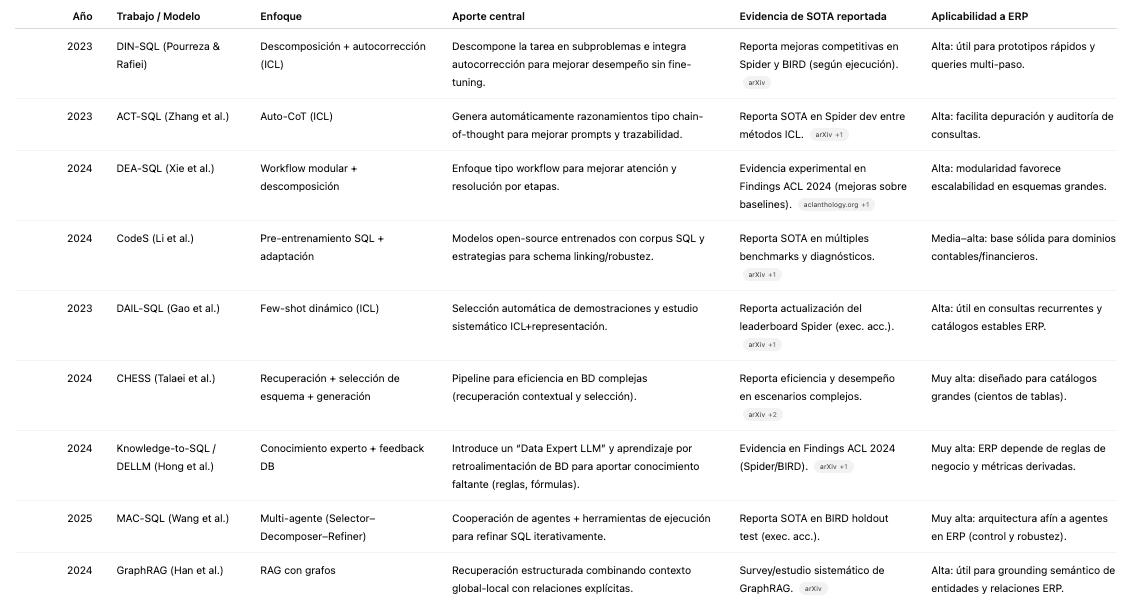
\includegraphics[width=\textwidth]{Tabla Estado del Arte.png}
	\caption{Comparación de metodologías del estado del arte en Text-to-SQL basadas en LLMs}
	\label{tab:estado_arte}
	\tablefont
	\textit{Nota.} Se presentan las principales características, enfoques técnicos y resultados de las metodologías más relevantes en la generación de SQL mediante modelos de lenguaje de gran escala. La tabla facilita la comparación entre los diferentes paradigmas estructurados que han marcado el avance reciente del campo.
\end{table*}
\subsection{Metodologías Basadas en LLMs para la Generación de SQL}

A diferencia de las aproximaciones tempranas basadas en reglas, plantillas o modelos de lenguaje preentrenados (PLMs), esta sección se concentra en las metodologías recientes que emplean grandes modelos de lenguaje (LLMs) como eje principal para la generación de SQL. Estos enfoques representan el estado del arte actual y se caracterizan por el uso de prompting especializado \cite{li2024comprehensive}, la descomposición modular de tareas \cite{xie2024dea, wang2025mac}, técnicas eficientes de ajuste fino \cite{li2024codes} y ciclos de retroalimentación iterativa que fortalecen la precisión y la capacidad de generalización entre dominios.

\subsubsection{Decomposition for Enhancing Attention (DEA-SQL)}

Xie et al. \cite{xie2024dea} introducen DEA-SQL, un enfoque de tipo workflow que descompone la tarea Text-to-SQL en pasos atómicos para focalizar la atención del LLM y mejorar su capacidad de resolución. El pipeline se organiza en cinco módulos: (1) Information Determination, que filtra ruido y selecciona atributos relevantes; (2) Classification \& Hint, que identifica el tipo de problema y ajusta prompts específicos; (3) SQL Generation, apoyado en few-shot prompting y plantillas; (4) Self-Correction, orientado a errores frecuentes como joins y agregaciones; y (5) Active Learning, que integra ejemplos fallidos para expandir el alcance del modelo.

Este diseño busca superar las limitaciones del single-step prompting, donde los prompts largos difunden la atención y afectan la precisión. En sus experimentos, DEA-SQL mejora entre 2 y 3 puntos porcentuales respecto a los baselines en Spider Dev, Spider-Realistic y BIRD Dev, y alcanza resultados state of the art en Spider Test \cite{xie2024dea}.

\subsubsection{DIN-SQL (Decomposed In-Context Learning with Self-Correction)}

DIN-SQL \cite{pourreza2023din} propone un enfoque basado completamente en in-context learning (ICL) que divide la tarea Text-to-SQL en subtareas guiadas por prompts especializados y añade un módulo de autocorrección para reparar errores comunes sin necesidad de ajuste fino. A partir del análisis de 500 ejemplos muestreados del conjunto de entrenamiento de Spider, los autores identifican seis categorías de fallos frecuentes: errores de schema linking, joins incompletos o incorrectos, uso inadecuado de GROUP BY, consultas con anidamiento y operaciones de conjuntos, SQL inválido y una categoría miscelánea.

Para mitigarlo, DIN-SQL incorpora una fase de autocorrección zero-shot, adaptada al tipo de modelo (prompts más fuertes para modelos medianos, más suaves para modelos avanzados), lo que permite mejorar la precisión sin reentrenamiento. A diferencia de DEA-SQL, su aporte principal no es alcanzar resultados state of the art, sino demostrar que una buena estructura de prompting—descomposición más verificación—puede acercar el rendimiento al de modelos ajustados mediante fine-tuning.

\subsubsection{MAC-SQL (Multi-Agent Collaborative Framework)}

Wang et al. \cite{wang2025mac} presentan MAC-SQL como un marco explícitamente multi-agente para Text-to-SQL, en el que la tarea se reparte entre tres roles complementarios. El Selector se encarga de reducir el espacio de búsqueda, identificando las partes del esquema más relevantes y construyendo sub-bases manejables. El Decomposer toma la pregunta original, la divide en subpreguntas y las resuelve de forma progresiva, lo que facilita el manejo de consultas largas o con múltiples condiciones. Por último, el Refiner ejecuta las consultas generadas, analiza los errores de ejecución y aplica correcciones iterativas.

En su configuración de referencia, MAC-SQL utiliza GPT-4 como backbone para establecer un ``upper bound'' de rendimiento y, a partir de ahí, ajusta por instrucciones SQL-Llama (7B, sobre Code Llama) para aproximar ese comportamiento con un modelo abierto. En el benchmark BIRD (test), MAC-SQL alcanza un 59.59\% de exactitud de ejecución, considerado state of the art en el momento de su publicación \cite{wang2025mac}.

\subsubsection{ACT-SQL (In-Context Learning con Chain-of-Thought Automático)}

ACT-SQL constituye una metodología reciente que busca potenciar la capacidad de razonamiento de los LLMs en la generación de SQL, mediante la incorporación de cadenas de razonamiento (chain-of-thought, CoT) generadas automáticamente \cite{zhang2023act}. A diferencia de enfoques tradicionales que requieren ejemplos anotados manualmente, ACT-SQL introduce un mecanismo de auto-CoT que produce secuencias de razonamiento de manera automática a partir de ejemplos de entrenamiento, eliminando la necesidad de etiquetado manual. Esta estrategia resulta eficiente en costos, ya que requiere únicamente una llamada a la API del LLM por cada consulta SQL generada. Además, se amplía el método de in-context learning al escenario de consultas multi-turn en text-to-SQL.

El método se apoya en tres pilares: (1) prompts orientados al esquema, que exploran distintas formas de representar tablas y relaciones; (2) selección híbrida de ejemplos (static exemplars, predefinidos y comunes a todas las consultas, y dynamic exemplars, seleccionados dinámicamente según similitud con la pregunta actual); y (3) generación automática de cadenas de razonamiento (CoT), que introduce pasos intermedios antes de producir la consulta final en SQL.

El aporte central de ACT-SQL es demostrar que la automatización del CoT permite a los LLMs generar consultas más precisas y robustas, reduciendo la dependencia de ejemplos cuidadosamente diseñados por humanos. Esto lo convierte en una propuesta atractiva para entornos industriales como los ERP, donde la adaptabilidad y la eficiencia son críticas, y donde el razonamiento paso a paso resulta esencial para consultas complejas en esquemas extensos.

\subsubsection{MCS-SQL (Multiple-Choice Selection with Multi-Prompts)}

Lee et al. \cite{lee2024mcs} proponen MCS-SQL como respuesta directa a un problema ampliamente documentado en los LLMs: su alta sensibilidad a los prompts. Cambios pequeños en la formulación del prompt pueden conducir a consultas SQL muy distintas, incluso cuando la intención del usuario es clara. Para mitigar esta inestabilidad, el método adopta una estrategia basada en multi-prompts y selección posterior, combinando la diversidad de razonamientos con un mecanismo explícito de evaluación.

El funcionamiento de MCS-SQL se organiza en dos etapas. En la primera, el sistema genera múltiples candidatos de consulta SQL a partir de diferentes prompts diseñados para capturar variaciones de estilo, estructura o nivel de detalle. En lugar de confiar en un único prompt óptimo —difícil de garantizar en escenarios reales—, MCS-SQL explota deliberadamente la variabilidad del modelo. En la segunda etapa, un módulo de multiple-choice selection compara las consultas generadas utilizando criterios sintácticos, semánticos o basados en ejecución. Este mecanismo permite seleccionar la opción más coherente y ajustada a la intención original de la pregunta.

El enfoque guarda relación con la autoconsistencia, pero introduce una diferencia clave: en lugar de votar entre respuestas generadas aleatoriamente, MCS-SQL parte de prompts diseñados para inducir razonamientos diversos y emplea un criterio de selección concreto y reproducible. En sus evaluaciones, el modelo alcanzó 89.6\% de exactitud en ejecución sobre Spider y resultados competitivos en BIRD, evidenciando que la diversidad guiada y la consolidación de hipótesis robustas son estrategias efectivas para contrarrestar la fragilidad de los LLMs ante variaciones de entrada.

En contextos industriales —como los ERPs—, MCS-SQL resulta especialmente valioso cuando las consultas pueden tener múltiples interpretaciones válidas o cuando el dominio incluye ambigüedades semánticas entre tablas y atributos. En estas situaciones, disponer de varias hipótesis SQL y un selector que determine cuál representa mejor la intención del usuario incrementa la confiabilidad del sistema y reduce errores críticos. Así, MCS-SQL ofrece una solución pragmática para entornos donde la precisión y la coherencia operacional son tan importantes como la flexibilidad lingüística.

\subsubsection{CHESS (Contextual Harnessing for Efficient SQL Synthesis)}

Talaei et al. \cite{talaei2024chess} introducen CHESS, un enfoque diseñado específicamente para contextos con esquemas grandes y complejos, donde enviar la totalidad del esquema al LLM resulta costoso e ineficiente. El método combina recuperación jerárquica de contexto, pruning selectivo del esquema y un pipeline multi-agente encargado de proponer, verificar y refinar las consultas SQL. En lugar de exponer al modelo a todas las tablas y columnas disponibles, CHESS identifica primero las partes más relevantes del esquema y construye, a partir de ellas, una vista reducida pero informativa para la generación de la consulta.

La principal fortaleza de CHESS es su eficiencia sin degradar el rendimiento: en esquemas de escala industrial su Schema Selector reduce en cinco veces los tokens procesados (con una mejora de exactitud cercana a 2 puntos), y en BIRD (test) alcanza un 71,10\% con cerca de un 83\% menos de llamadas al LLM \cite{talaei2024chess}. Esta combinación de selección contextual y cooperación entre agentes resulta especialmente pertinente para entornos ERP, donde los esquemas suelen abarcar cientos de tablas y atributos. En estos escenarios, CHESS ofrece una vía concreta para equilibrar el costo computacional con la necesidad de preservar suficiente cobertura semántica para responder preguntas empresariales complejas.

Los análisis comparativos de Shi et al. \cite{shi2025comprehensive} y Liu et al. \cite{liu2025survey} sitúan a modelos como DEA-SQL, DAIL-SQL \cite{gao2024dail}, MAC-SQL, ACT-SQL, MCS-SQL y CHESS dentro de los llamados ``paradigmas estructurados'', caracterizados por organizar la generación de SQL en fases claras, apoyarse en contexto recuperado de forma controlada y, en muchos casos, distribuir el razonamiento entre varios agentes. Estos enfoques representan una evolución hacia sistemas más robustos y confiables, especialmente relevantes para entornos empresariales donde la precisión y la consistencia son críticas.


\section{Arquitectura Propuesta}

\begin{figure*}[t]
	\centering
	\includegraphics[width=\textwidth]{Arquitectura.jpg}
	\caption{Arquitectura propuesta multi-agente para Text-to-SQL en el ERP Fail Fast. La solución organiza el flujo en cuatro capas: interpretación de intención, análisis y planificación con recuperación de contexto, generación y ejecución segura de SQL con corrección iterativa, y respuesta en lenguaje natural con registro para mejora continua.}
	\label{fig:failfast_text2sql_arch}
\end{figure*}

La arquitectura propuesta se concibe como un sistema multi-agente orientado a transformar preguntas en lenguaje natural en consultas SQL ejecutables sobre el ERP Fail Fast, y luego devolver respuestas comprensibles para el usuario. Se inspira en los paradigmas estructurados descritos en el estado del arte —especialmente MAC-SQL para la colaboración multi-agente, DIN-SQL para la descomposición de consultas y DEA-SQL para la planificación— adaptados a un entorno real.

A alto nivel, la arquitectura implementa un marco colaborativo multi-agente donde cada agente tiene responsabilidades específicas y bien definidas, organizándose en cuatro capas funcionales: entrada e interpretación de la intención, análisis y planificación de la consulta, generación y ejecución de SQL, respuesta en lenguaje natural y retroalimentación.


\subsection{Capa de Entrada e Interpretación de la Intención}

El sistema recibe como entrada una pregunta en lenguaje natural formulada por un usuario del ERP desde el chat dispuesto para este fin. Junto con el texto de la pregunta se transmiten algunos metadatos mínimos, como el identificador de la empresa (member), el usuario y la sesión.

Sobre esta entrada actúa un agente de intención basado en un LLM, cuyo objetivo no es generar SQL, sino:
\begin{itemize}
	\item Entender qué está preguntando el usuario (ventas, inventarios, compras, nómina, etc.)
	\item Decidir si la solicitud requiere realmente acceder a la base de datos mediante SQL o puede resolverse con una explicación directa
	\item Mantener un diálogo coherente, pidiendo aclaraciones cuando la pregunta es ambigua o incompleta
\end{itemize}

Solo cuando la intención está clara y se trata de una consulta sobre datos del ERP, este agente ``enciende'' el modo Text-to-SQL y pasa la petición a la siguiente capa. Este \emph{gating} conversacional constituye una contribución diferencial de este trabajo: marcos multi-agente como MAC-SQL \cite{wang2025mac} filtran el \emph{esquema} (su Selector poda tablas y columnas irrelevantes) pero asumen que toda entrada es una consulta válida; aquí se filtra la \emph{intención} antes de exponer la base de datos.

\subsection{Capa de Análisis y Planificación de la Consulta}

Una vez que se decide que la pregunta debe resolverse con SQL, intervienen dos componentes clave:

\subsubsection{Agente de Descomposición (inspirado en DIN-SQL)}

El primer componente es un agente de descomposición, alineado con las ideas de DIN-SQL \cite{pourreza2023din}. Su función es tomar la pregunta del usuario y producir una representación más estructurada, que incluye:
\begin{itemize}
	\item Una reformulación clara de la intención (``El usuario desea obtener...'')
	\item Una lista de pasos lógicos necesarios para responderla (qué tablas parecen relevantes, qué filtros temporales o de estado, si se requieren agregaciones o agrupaciones, etc.)
	\item Una clasificación de complejidad (fácil, media, compleja) en función del número de tablas y la necesidad de joins.
\end{itemize}

Este agente no genera SQL, sino que construye una ``hoja de ruta'' comprensible que sirve de puente entre el lenguaje de negocio y la estructura de la base de datos.

En esta arquitectura, cada pregunta se clasifica en tres niveles de complejidad: fácil, media, compleja. Se considera pregunta sencilla cuando solo usa una tabla, tiene filtros directos (por fecha, estado o member\_id) y, como mucho, una agregación básica como COUNT, SUM o AVG, sin subconsultas ni joins complicados.

Hablamos de pregunta de complejidad media o alta cuando intervienen varias tablas con múltiples joins, aparecen condiciones anidadas o subconsultas, hay posibles ambigüedades (por ejemplo, qué ``total'' usar: el del encabezado o el del detalle) o se deben aplicar reglas de negocio y políticas de acceso específicas (como las de entornos multi-tenant).

Esta clasificación, inspirada en los enfoques de descomposición y enrutamiento por tipo de problema \cite{pourreza2023din, xie2024dea}, es la que define si la pregunta sigue un flujo directo de generación de SQL o un pipeline más elaborado con planificación y agentes especializados.

\subsubsection{Recuperación de Contexto y Planificación (inspirado en DEA-SQL y DAIL-SQL)}

Con la descomposición en la mano, la arquitectura consulta un módulo de recuperación de contexto basado en búsqueda vectorial:
\begin{itemize}
	\item Recupera fragmentos de documentación del esquema (tablas, columnas, descripciones) mediante búsqueda por similitud semántica
	\item Recupera ejemplos históricos de preguntas y consultas SQL similares mediante búsqueda vectorial en una base de conocimiento
	\item Combina ambos tipos de contexto para proporcionar información relevante al planificador
\end{itemize}

A partir de este contexto recuperado y de la descomposición anterior, entra en juego un agente planificador de SQL inspirado en DEA-SQL \cite{xie2024dea}. Este agente:
\begin{itemize}
	\item Valida qué partes del esquema del ERP son realmente relevantes para la consulta
	\item Propone uno o varios planes de consulta (qué tablas unir, qué filtros aplicar, cómo agrupar)
	\item Explica, a nivel interno del sistema, la lógica de cada plan
\end{itemize}

\subsection{Capa de Generación y Ejecución de SQL}

Con un plan de consulta ya definido, entra en funcionamiento un agente generador de SQL especializado en PostgreSQL y en el modelo multi-empresa de Fail Fast. Este agente:

\begin{itemize}
	\item Recibe la intención original del usuario, la descomposición estructurada y el plan de consulta
	\item Genera una consulta SQL directa basada en las reglas de negocio del ERP
	\item Implementa un sistema de corrección iterativa que permite refinar la consulta en caso de errores de ejecución
\end{itemize}

El agente tiene reglas estrictas de seguridad y contexto:
\begin{itemize}
	\item Solo puede producir consultas de lectura (SELECT)
	\item Debe respetar el contexto de la empresa (incluyendo condiciones como member\_id)
	\item Debe limitar el volumen de resultados (uso de LIMIT) para evitar respuestas inmanejables
	\item No puede inventar tablas o columnas que no existan
	\item Incluye filtros obligatorios para excluir registros borrados (audit\_status)
\end{itemize}

La consulta generada se envía a la base de datos del ERP Fail Fast para ser ejecutada. Si la ejecución produce errores, esa información se devuelve al agente generador, que intenta corregir la consulta hasta tres iteraciones. Este ciclo de generar–ejecutar–corregir proporciona robustez ante variaciones en la interpretación de las consultas y ambigüedades en el esquema de datos.

\subsection{Capa de Respuesta en Lenguaje Natural y Retroalimentación}

Cuando la consulta SQL se ejecuta correctamente, el sistema obtiene un conjunto de resultados estructurados (filas, columnas, JOINS) que no son adecuados para mostrarse directamente a cualquier usuario. Para ello se utiliza un agente de respuesta que:
\begin{itemize}
	\item Recibe la pregunta original, la descomposición y los resultados de la base de datos
	\item Resume y explica los resultados en el mismo idioma en el que el usuario preguntó
	\item Presenta los datos de forma amigable (por ejemplo, en forma de listado o tabla)
	\item Evita exponer identificadores internos o detalles técnicos irrelevantes
\end{itemize}

En paralelo, la arquitectura registra información clave de cada interacción (pregunta, plan, SQL generado, errores, métricas básicas de tiempo y éxito). Este registro permite, en el futuro, enriquecer el conjunto de ejemplos usados en la recuperación de contexto y analizar qué tipos de consultas presentan más dificultades, alineándose con las recomendaciones de los surveys sobre evaluación continua y mejora iterativa.

\subsection{Relación con el Estado del Arte}

En conjunto, la arquitectura:
\begin{itemize}
	\item Implementa el marco colaborativo multi-agente de MAC-SQL, distribuyendo la tarea Text-to-SQL entre agentes especializados que colaboran para resolver consultas complejas
	\item Retoma de DIN-SQL la idea de descomponer la pregunta y analizar la complejidad antes de generar SQL
	\item Toma de DEA-SQL la noción de un planificador que organiza la atención del modelo sobre el esquema
	\item Se beneficia del enfoque de DAIL-SQL al usar recuperación basada en ejemplos relevantes y documentación de esquema
	\item Materializa un flujo multi-agente que distribuye las responsabilidades entre varios componentes especializados (intención, descomposición, planificación, generación, respuesta), en vez de delegar todo en un único LLM monolítico
\end{itemize}

Todo ello se implementa sobre el ERP Fail Fast, cuya base de datos fue diseñada de forma documentada y con una nomenclatura pensada para ser interpretable por modelos de lenguaje, lo que facilita el schema linking y la comprensión de la intención del usuario en términos de tablas y columnas.




\section{Metodología}

\subsection{Diseño metodológico}

La presente investigación adopta un enfoque experimental cuantitativo, orientado a evaluar el impacto individual y combinado de distintos componentes arquitectónicos en la tarea de generación de consultas SQL a partir de lenguaje natural (Text-to-SQL) dentro de un sistema ERP real. El diseño experimental se fundamenta en un estudio controlado con análisis de ablación, técnica ampliamente utilizada para estimar la contribución de módulos específicos dentro de arquitecturas complejas basadas en modelos de lenguaje, particularmente en escenarios donde múltiples etapas de razonamiento y componentes interactúan de manera no trivial \cite{wang2025mac}.

Con el fin de facilitar la experimentación sistemática, la reproducibilidad y la orquestación controlada de configuraciones arquitectónicas, la implementación experimental se realizó utilizando n8n como plataforma de automatización y orquestación de flujos, en línea con el uso de plataformas low-code para NL-to-SQL \cite{aparicio2023natural}. Esta herramienta permitió definir de manera declarativa y parametrizable cada configuración experimental, habilitando o deshabilitando componentes arquitectónicos —como RAG, memoria, clasificación de intención y descomposición— sin modificar el código base del sistema. El uso de n8n resulta particularmente adecuado en este contexto, ya que posibilita la instrumentación precisa de pipelines de inferencia complejos, el registro automático de métricas y la repetición homogénea de experimentos bajo condiciones controladas.

Asimismo, la evaluación se llevó a cabo empleando modelos de lenguaje de la familia Gemini 2.5, específicamente Gemini 2.5 Flash, Gemini 2.5 Flash-Lite y Gemini 2.5 Pro, seleccionados con el objetivo de analizar el comportamiento del sistema bajo distintos perfiles de capacidad, latencia y costo computacional. Esta elección permite estudiar no solo el impacto arquitectónico, sino también la robustez del diseño propuesto frente a variaciones en la capacidad del modelo subyacente, aspecto crítico en entornos empresariales donde existen restricciones operativas y económicas. Todos los modelos fueron utilizados en modalidad de inferencia consistente, manteniendo constantes los prompts base y las estrategias de generación, con el fin de aislar los efectos atribuibles exclusivamente a la arquitectura.
A diferencia de evaluaciones tradicionales centradas únicamente en comparar sistemas completos como "cajas negras", este trabajo evalúa configuraciones parciales de la arquitectura, habilitando o deshabilitando componentes de forma sistemática con el fin de aislar su efecto sobre métricas clave. Este enfoque permite responder no solo si la arquitectura mejora el desempeño, sino también por qué y qué componentes aportan mayor valor en escenarios empresariales reales.

\subsection{Conjunto de consultas de referencia (Gold Queries)}

Para garantizar una evaluación precisa y reproducible, se construyó un conjunto de 53 consultas de referencia (gold queries), elaboradas manualmente por expertos con conocimiento del esquema de datos del ERP Fail Fast. Cada consulta gold incluye:

\begin{itemize}
	\item Una pregunta en lenguaje natural formulada desde la perspectiva de un usuario empresarial.
	\item Una consulta SQL ejecutable y validada sobre la base de datos real del sistema.
	\item La verificación de que el resultado retornado corresponde fielmente a la intención semántica de la pregunta.
\end{itemize}

La construcción manual de estas consultas minimiza ambigüedades propias de conjuntos sintéticos o genéricos y asegura que la evaluación refleje casos reales de uso empresarial. En Text-to-SQL, la validación por ejecución es una práctica consolidada, dado que la corrección funcional depende de la equivalencia semántica del resultado más que de la coincidencia textual del SQL \cite{scholak2021picard, hong2024bird}.

\subsection{Componentes arquitectónicos evaluados}

La arquitectura propuesta se diseñó de forma modular y parametrizable, permitiendo activar o desactivar componentes específicos durante la inferencia con el fin de analizar su impacto individual y combinado sobre el desempeño del sistema mediante un estudio sistemático de ablación. En esta sección, cada componente se define desde una perspectiva operacional, es decir, en términos de cómo modifica el flujo de generación de SQL cuando está activo.

\textbf{RAG (Retrieval-Augmented Generation).} Cuando está activo, el sistema incorpora al prompt de generación información recuperada dinámicamente, incluyendo descripciones del esquema, relaciones semánticas y reglas de negocio relevantes para la consulta. Cuando está desactivado, la generación de SQL se realiza únicamente a partir de la pregunta del usuario y el prompt base.

\textbf{Memoria.} Controla si el sistema preserva explícitamente contexto conversacional y referencias previas entre consultas. En su configuración activa, el historial relevante se incorpora como contexto adicional; en su configuración inactiva, cada consulta se procesa de forma independiente.

\textbf{Intención (Intent Classification).} Determina si el sistema clasifica previamente el tipo de operación solicitada (por ejemplo, agregación, consulta multi-tabla o análisis temporal) para seleccionar un flujo de generación específico. Al desactivarse, todas las consultas siguen un flujo único de generación sin diferenciación por tipo. esto en realidad lo que hace es: Esta lo que hace es determinar si se puede responder directamente la pregunta mediante Sql o por el contrario la pregunta es muy pobre o ambigua para que se pueda responder.

\textbf{DIN (Decomposition-In-Natural-Language).} Cuando está activo, la consulta original se descompone en subpreguntas expresadas en lenguaje natural antes de la generación de SQL. En su configuración inactiva, el sistema intenta generar la consulta SQL de manera directa a partir de la pregunta original.

\textbf{DEA (Decomposition-Execution-Aware).} Habilita un esquema de generación orientado a la ejecutabilidad, en el que la salida se estructura para facilitar validación posterior por ejecución (p. ej., priorizando consistencia de esquema, restricciones y composición de operadores) y para producir consultas más robustas frente a errores comunes en bases de datos reales. En esta arquitectura, DEA no realiza directamente la autocorrección: su rol es guiar la generación hacia SQL ejecutable y modular, mientras que la ejecución y los ciclos de corrección iterativa —cuando están habilitados— son responsabilidad del componente de ejecución y refinamiento (p. ej., Executor/Refiner). Al desactivarse DEA, el sistema mantiene la generación de SQL, pero sin aplicar este sesgo explícito hacia ejecutabilidad durante la construcción de la consulta.
Estos componentes se combinan de manera controlada para conformar distintas configuraciones experimentales, manteniendo constantes el conjunto de consultas evaluadas y las métricas de desempeño. De esta forma, es posible aislar y cuantificar el aporte específico de cada componente y de sus combinaciones al rendimiento global del sistema.

\subsection{Espacio experimental y combinaciones evaluadas}

Dado un conjunto de cinco componentes binarios (activo/inactivo), el espacio total de configuraciones posibles corresponde a:

$$2^5 - 1 = 31$$

Se excluyó la configuración nula (sin componentes activos), dado que no produce generación SQL. De este espacio de 31 combinaciones posibles se evaluaron efectivamente 19 configuraciones, priorizando aquellas que incorporan recuperación contextual (RAG) —requisito para generar SQL válido sobre el esquema del ERP— junto con un conjunto de configuraciones de contraste sin RAG. Entre las configuraciones evaluadas se incluyen:

\begin{itemize}
	\item RAG
	\item Intención
	\item DIN
	\item DEA
	\item RAG + Intención
	\item Intención + DIN + DEA
	\item RAG + Intención + DIN + DEA
	\item RAG + Memoria + Intención + DIN + DEA (arquitectura completa)
\end{itemize}

Cada configuración fue ejecutada sobre el mismo conjunto de consultas de referencia, garantizando condiciones experimentales homogéneas.

\subsection{Conjuntos de datos de evaluación}
\label{sec:datasets}

La evaluación se apoya en dos conjuntos complementarios, ambos anclados al esquema real del ERP Fail Fast. El \textbf{conjunto de un solo turno} (ablación) es el banco de preguntas empresariales de complejidad media y compleja; cada registro asocia una pregunta en lenguaje natural con su descomposición, las tablas y columnas relevantes y una consulta SQL de referencia (gold) validada por ejecución, distribuidas en tres niveles (Fácil, Media, Compleja) y cubriendo agregaciones financieras, consultas multi-tabla, análisis temporal y reportes operativos. Este conjunto se ejecutó bajo cada una de las 19 configuraciones evaluadas.

El \textbf{conjunto conversacional multi-turno}, construido para evaluar los módulos de Intensión y Memoria, comprende \textbf{100 conversaciones} (hasta 10 turnos; \textbf{759 turnos} en total) derivadas de las preguntas anteriores. El orden de los turnos es significativo: cada conversación encadena un turno inicial ejecutable con seguimientos que dependen del contexto acumulado (referencias elípticas como ``ahora el promedio'', ``ordénalo'', ``¿a qué tipo pertenece?''), intercalados con turnos puramente conversacionales que \emph{no} deben disparar SQL y turnos ambiguos que deben motivar una aclaración (446 turnos ejecutables, 196 conversacionales y 117 ambiguos).

Sobre el conjunto de un solo turno se calculan Execution Accuracy, Component Matching y Time-to-Answer. Sobre el conjunto conversacional, la evaluación reproduce el flujo agentivo completo (RAG+Memoria+Intensión+DIN+DEA) contra la base de datos de prueba, con memoria persistente entre turnos: se registra la acción tomada por el sistema (ejecutar SQL, responder conversacionalmente o pedir aclaración) y, cuando ejecuta SQL, la consulta se ejecuta realmente y su resultado se compara con el de referencia mediante Execution Accuracy normalizada. Esto mide dos capacidades propias del escenario conversacional: el \emph{gating} de intención (cuándo ejecutar SQL) y la \emph{resolución de contexto} (reconstruir la consulta desde la memoria de turnos previos).

\subsection{Métricas de evaluación}

El desempeño de cada configuración se evaluó utilizando tres métricas complementarias, ampliamente aceptadas en la literatura Text-to-SQL y pertinentes para el contexto ERP.

\subsubsection{Execution Accuracy (EX)}

Mide el porcentaje de consultas cuya ejecución retorna exactamente el mismo resultado que la consulta gold correspondiente, independientemente de la forma sintáctica del SQL. Esta métrica es especialmente relevante en entornos empresariales, donde la corrección semántica del resultado es prioritaria frente a la coincidencia textual \cite{yu2018spider, hong2024bird}.

\subsubsection{Component Matching (CM)}

Evalúa el grado de coincidencia entre componentes estructurales del SQL generado y el SQL gold, tales como:

\begin{itemize}
	\item Tablas utilizadas
	\item Columnas seleccionadas
	\item Operaciones de agregación
	\item Cláusulas de filtrado y agrupación
\end{itemize}

Esta métrica permite identificar errores parciales que no siempre se reflejan en la ejecución final, proporcionando una visión más granular del comportamiento del modelo.

\subsubsection{Tiempo de respuesta (Time-to-Answer, TTA)}

Corresponde al tiempo total transcurrido desde que el usuario formula la consulta en lenguaje natural hasta que el sistema retorna el resultado final. La literatura reporta latencias muy dispares entre metodologías y destaca los escenarios interactivos de baja latencia \cite{liu2025survey}; su proyección a sistemas ERP, donde la latencia condiciona la experiencia del usuario y la viabilidad operativa, es un aporte de este trabajo.

\subsection{Procedimiento experimental}

El procedimiento seguido para cada configuración fue el siguiente:

\begin{enumerate}
	\item Selección de una configuración específica de componentes.
	\item Ejecución secuencial del conjunto de consultas de referencia bajo dicha configuración.
	\item Registro automático del SQL generado, resultado de ejecución, componentes estructurales y tiempo de respuesta.
	\item Cálculo agregado de las métricas EX, CM y TTA.
	\item Repetición del proceso para las 19 configuraciones evaluadas.
\end{enumerate}

Este procedimiento garantiza comparabilidad directa entre configuraciones y permite analizar tanto el impacto individual de cada componente como sus efectos combinados.

\subsection{Análisis del impacto de componentes}

Finalmente, los resultados obtenidos permiten realizar un análisis de impacto por componente mediante:

\begin{itemize}
	\item Comparación directa entre configuraciones que difieren en un único componente.
	\item Identificación de sinergias entre módulos (por ejemplo, RAG + descomposición).
	\item Evaluación de compromisos (trade-offs) entre precisión y tiempo de respuesta.
\end{itemize}

Este análisis constituye la base empírica para determinar qué componentes son esenciales, cuáles son complementarios y en qué escenarios su inclusión resulta más beneficiosa, aportando evidencia experimental sólida para el diseño de arquitecturas Text-to-SQL en sistemas ERP.

\subsection{Referencia al anexo del conjunto de consultas}

Con el fin de preservar la claridad del capítulo metodológico sin sacrificar trazabilidad ni reproducibilidad, el detalle completo del conjunto de consultas —incluyendo la pregunta en lenguaje natural, la clasificación por complejidad, la descomposición semántica, las tablas y columnas relevantes del esquema y la consulta SQL de referencia— se presenta en el Anexo A.

\section{Resultados Experimentales y Discusión}

En este capítulo se presentan los resultados del estudio experimental realizado mediante un análisis de ablación sobre distintas configuraciones arquitectónicas del sistema de transformación de lenguaje natural a SQL propuesto. Todas las configuraciones fueron evaluadas bajo condiciones controladas sobre un conjunto fijo de 53 preguntas de referencia, lo que permite comparar de manera directa el efecto individual y combinado de cada módulo sobre el desempeño del sistema.

El análisis se estructura en torno a cuatro dimensiones complementarias: (1) la calidad estructural del SQL generado, (2) la exactitud por ejecución, (3) la robustez ante errores considerando mecanismos de corrección, y (iv) la capacidad real de generación correcta desde el primer intento, sin recurrir a autocorrección. Esta descomposición permite evaluar no solo si el sistema logra producir consultas funcionales, sino también cómo y bajo qué condiciones se alcanza dicho desempeño.

Para ello, se emplean métricas consolidadas en la literatura de Text-to-SQL. En particular, se reporta el promedio del F1-score de Component Matching para los componentes SELECT, WHERE, GROUP BY y KEYWORDS, con el fin de medir el grado de alineamiento estructural entre el SQL generado y el SQL de referencia. Adicionalmente, se utiliza Execution Accuracy, que evalúa la corrección semántica de la consulta a partir del resultado de su ejecución. Finalmente, se incorporan dos métricas orientadas a robustez: SIN ERRORES, que cuantifica el éxito considerando mecanismos de reparación durante la ejecución, y SIN\_AUTO\_CORRECCION, que estima la proporción de consultas correctamente generadas desde el primer intento. En conjunto, estas métricas permiten caracterizar el desempeño del sistema desde una perspectiva estructural, funcional y operativa.

\begin{figure}[htbp]
	\centering
	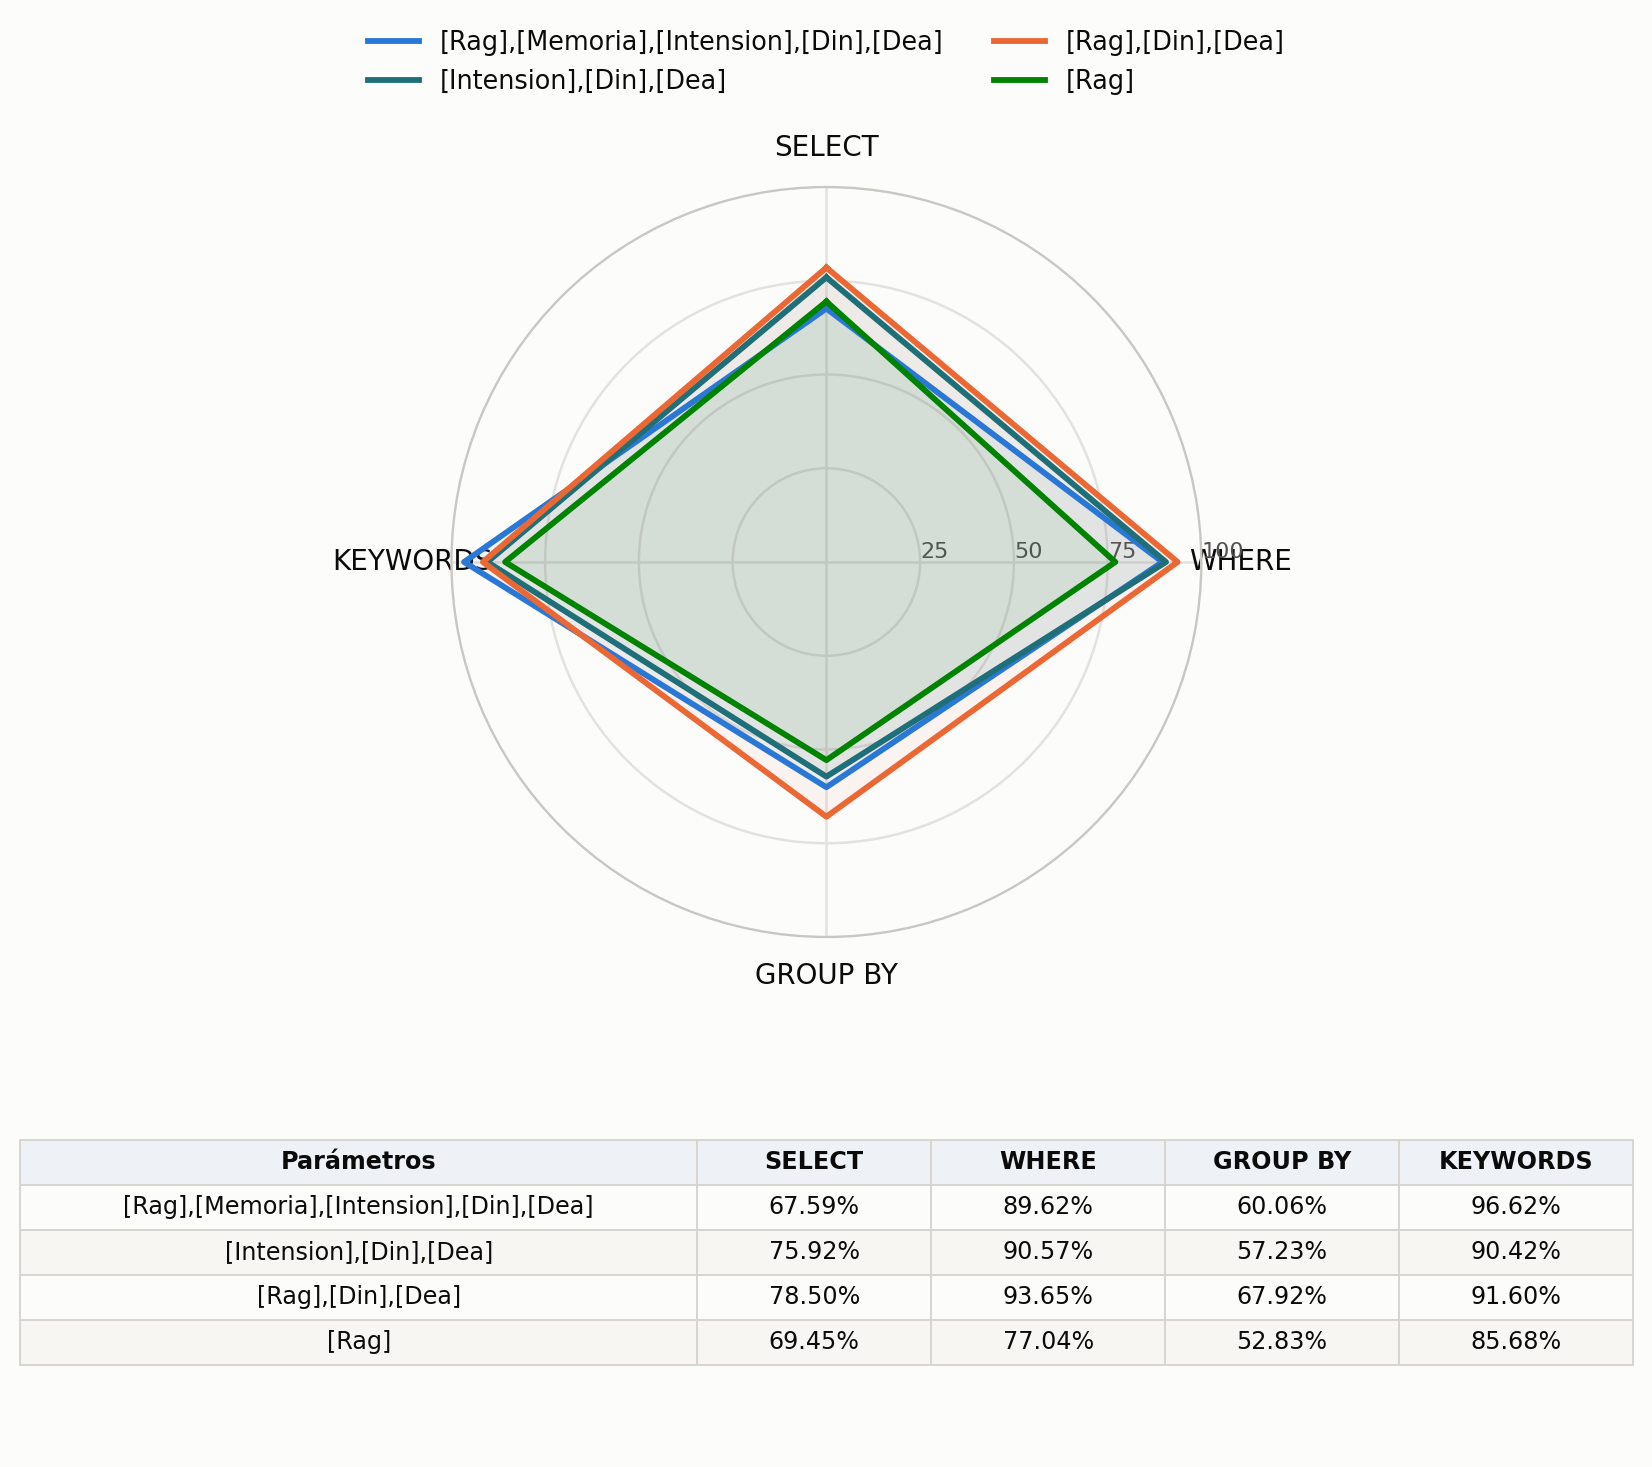
\includegraphics[width=0.9\linewidth]{Figura 5.1 - SQL.png}
	\caption{Comparación entre Component Matching y Execution Accuracy para distintas configuraciones arquitectónicas. Esta gráfica permite visualizar que un alto Component Matching no garantiza, por sí solo, una ejecución correcta del SQL.}
	\label{fig:component_matching_vs_execution}
\end{figure}

Asimismo, se observa que configuraciones con diferentes combinaciones de módulos pueden alcanzar valores similares de Component Matching, aun cuando su desempeño en ejecución difiere significativamente. Este resultado sugiere que una alta correspondencia estructural, si bien es una condición necesaria, no garantiza por sí sola la generación de consultas SQL funcionales. La Figura~\ref{fig:component_matching_vs_execution} ilustra claramente esta disociación entre calidad estructural y corrección funcional.

\subsection{Calidad estructural del SQL (Component Matching)}

Los resultados correspondientes a la métrica de Component Matching muestran que la mayoría de las configuraciones evaluadas alcanzan altos niveles de correspondencia estructural, especialmente en los componentes SELECT y WHERE, donde los valores promedio de F1-score superan frecuentemente el 85\%. Este comportamiento indica que el sistema es capaz de identificar de forma consistente las columnas relevantes y las condiciones de filtrado implícitas o explícitas en las preguntas formuladas en lenguaje natural.

En contraste, el componente GROUP BY presenta valores sistemáticamente inferiores en comparación con SELECT y WHERE. Esta tendencia se mantiene a lo largo de todas las configuraciones evaluadas y es consistente con observaciones previas en la literatura, donde las operaciones de agregación suelen encontrarse implícitas en el lenguaje natural y requieren un mayor nivel de inferencia semántica y estructural. En particular, la correcta identificación de la clave de agrupación resulta más sensible a ambigüedades del dominio y a la necesidad de conocimiento contextual adicional.


\subsection{Exactitud de ejecución (Execution Accuracy)}

La métrica de Execution Accuracy revela diferencias sustanciales entre las configuraciones arquitectónicas evaluadas. En particular, se observa que algunas configuraciones que presentan altos valores de Component Matching experimentan una caída significativa en exactitud por ejecución, lo que evidencia que la correcta identificación de componentes estructurales no siempre se traduce en consultas semánticamente correctas y ejecutables.

Un caso representativo es la configuración [Intensión + DIN + DEA], que alcanza valores elevados de F1-score en el componente WHERE, pero obtiene una Execution Accuracy del 37,74\%. Este resultado indica que, aun cuando el razonamiento estructural es adecuado, la ausencia de un mecanismo explícito de grounding contextual limita la capacidad del sistema para seleccionar tablas, columnas o relaciones correctas dentro de un esquema complejo.

Por el contrario, la configuración [RAG + DIN + DEA] alcanza el mejor desempeño global, con una Execution Accuracy superior al 81\%, superando incluso configuraciones más complejas que incorporan módulos adicionales como Memoria o clasificación explícita de Intensión. Este comportamiento sugiere que la recuperación contextual del esquema cumple un rol determinante en la traducción efectiva de la intención del usuario a consultas SQL ejecutables, particularmente en entornos empresariales con esquemas extensos.

\begin{figure}[htbp]
	\centering
	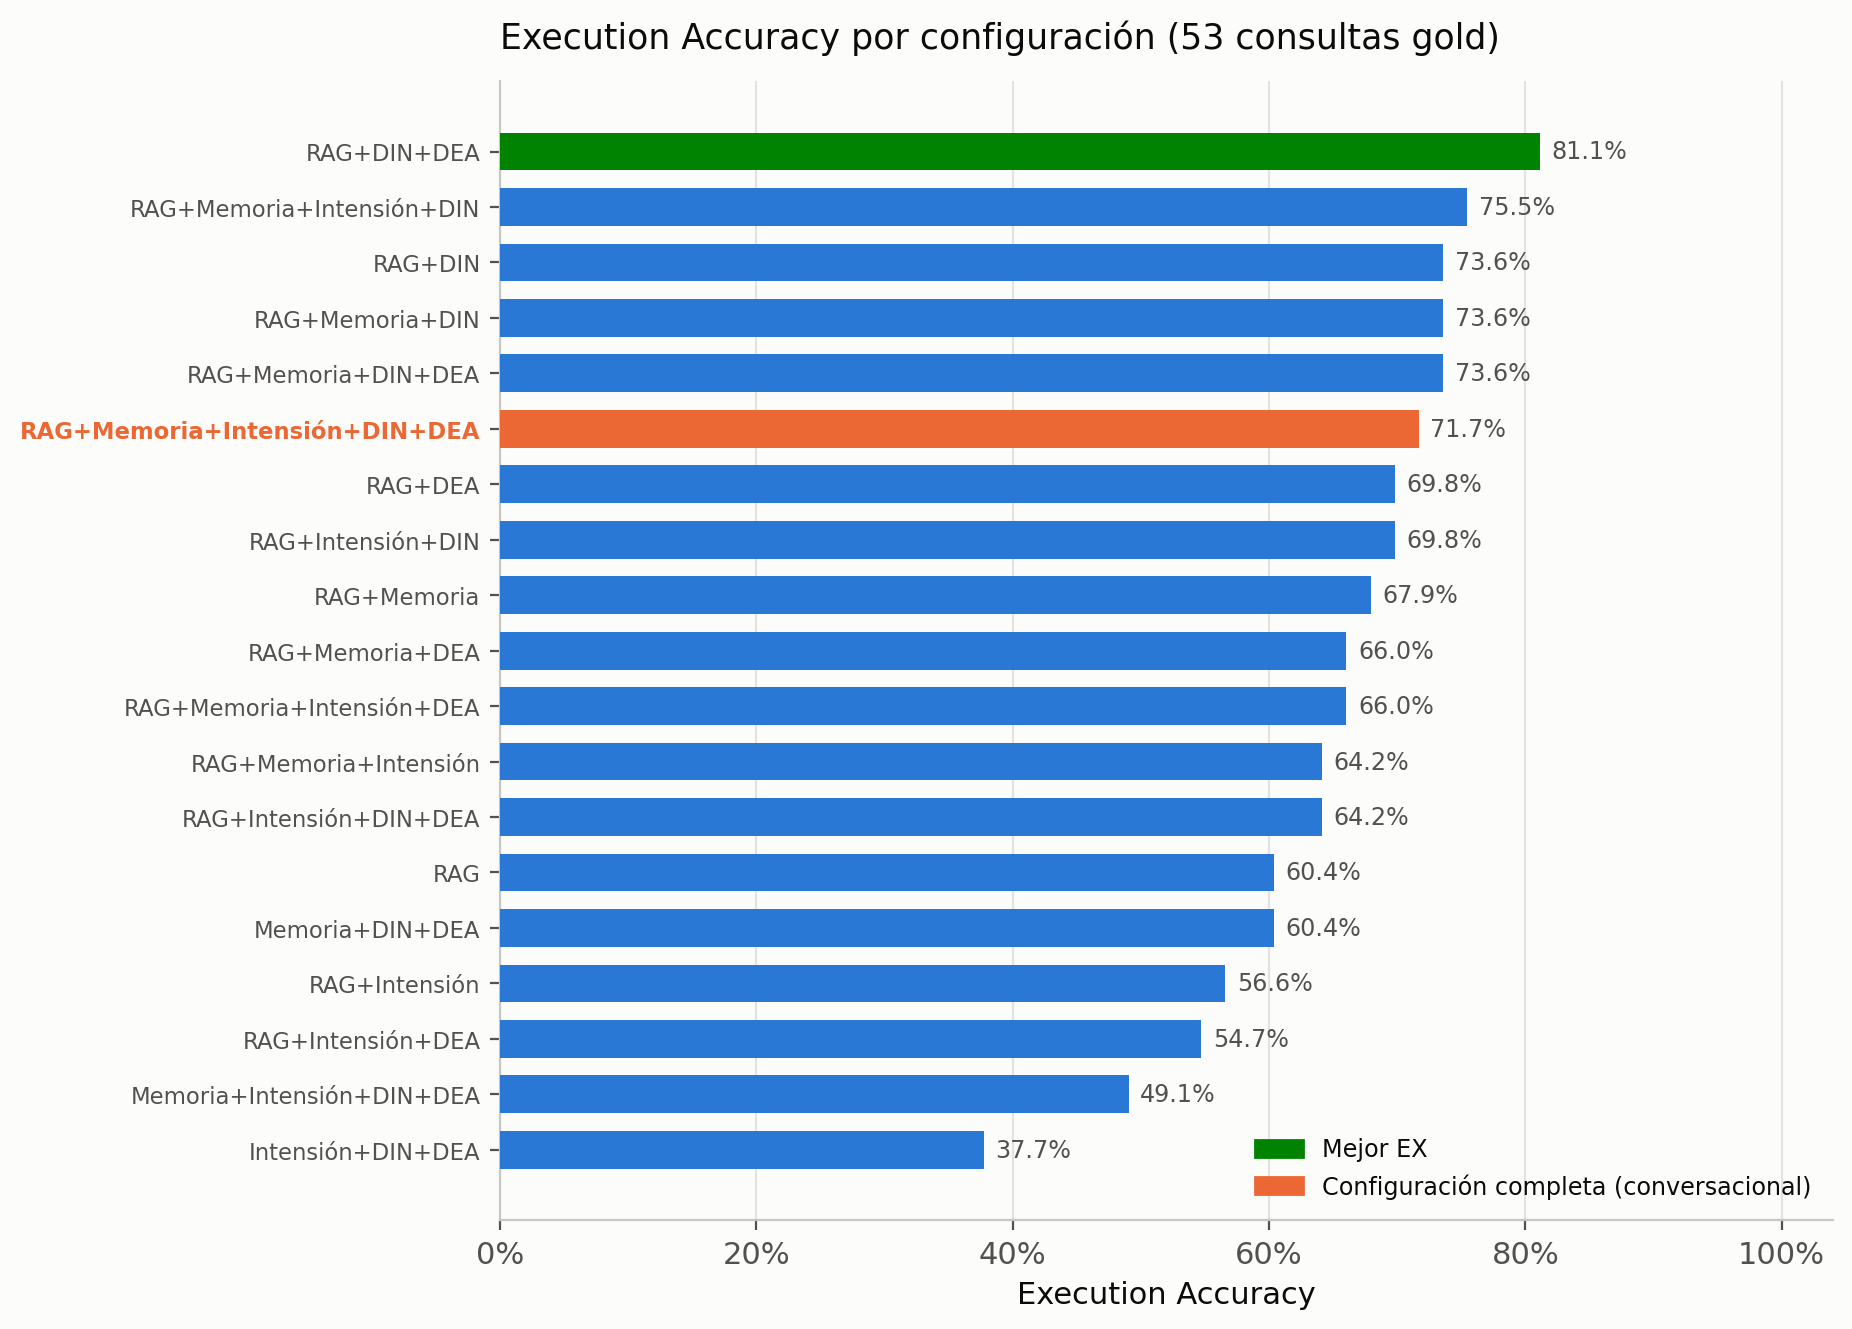
\includegraphics[width=\linewidth]{Figura 5.2 - Ranking EX 19 configuraciones.png}
	\caption{Exactitud de ejecución (Execution Accuracy) para las 19 configuraciones arquitectónicas evaluadas sobre las mismas 53 consultas gold. Se observan diferencias sustanciales entre configuraciones, destacando el rol determinante de la recuperación contextual del esquema (RAG); se resalta la configuración completa seleccionada para el escenario conversacional.}
	\label{fig:execution_accuracy}
\end{figure}

En conjunto, estos resultados evidencian una brecha clara entre calidad estructural y corrección funcional, resaltando la necesidad de evaluar explícitamente la ejecución para caracterizar el desempeño real de sistemas Text-to-SQL. La Figura~\ref{fig:execution_accuracy} presenta de manera visual las diferencias de rendimiento entre las configuraciones evaluadas.

\subsection{Robustez ante errores considerando autocorrección (SIN ERRORES)}

La métrica SIN ERRORES evalúa la capacidad del sistema para producir una consulta funcional considerando la presencia de mecanismos de ajuste y corrección automática durante la generación y ejecución del SQL. Los resultados muestran que la mayoría de las configuraciones que incorporan RAG alcanzan valores cercanos o iguales al 100\%, lo que evidencia una alta robustez frente a errores sintácticos, referencias incorrectas o fallos menores en la formulación de la consulta.

Este comportamiento indica que la recuperación aumentada por contexto no solo mejora la comprensión semántica de la consulta, sino que también actúa como un mecanismo de mitigación de errores, reduciendo la probabilidad de fallos no recuperables durante la ejecución. En particular, el acceso a descripciones del esquema y ejemplos relevantes parece facilitar la corrección iterativa de errores comunes, como joins incompletos o uso incorrecto de agregaciones.

\begin{figure}[htbp]
	\centering
	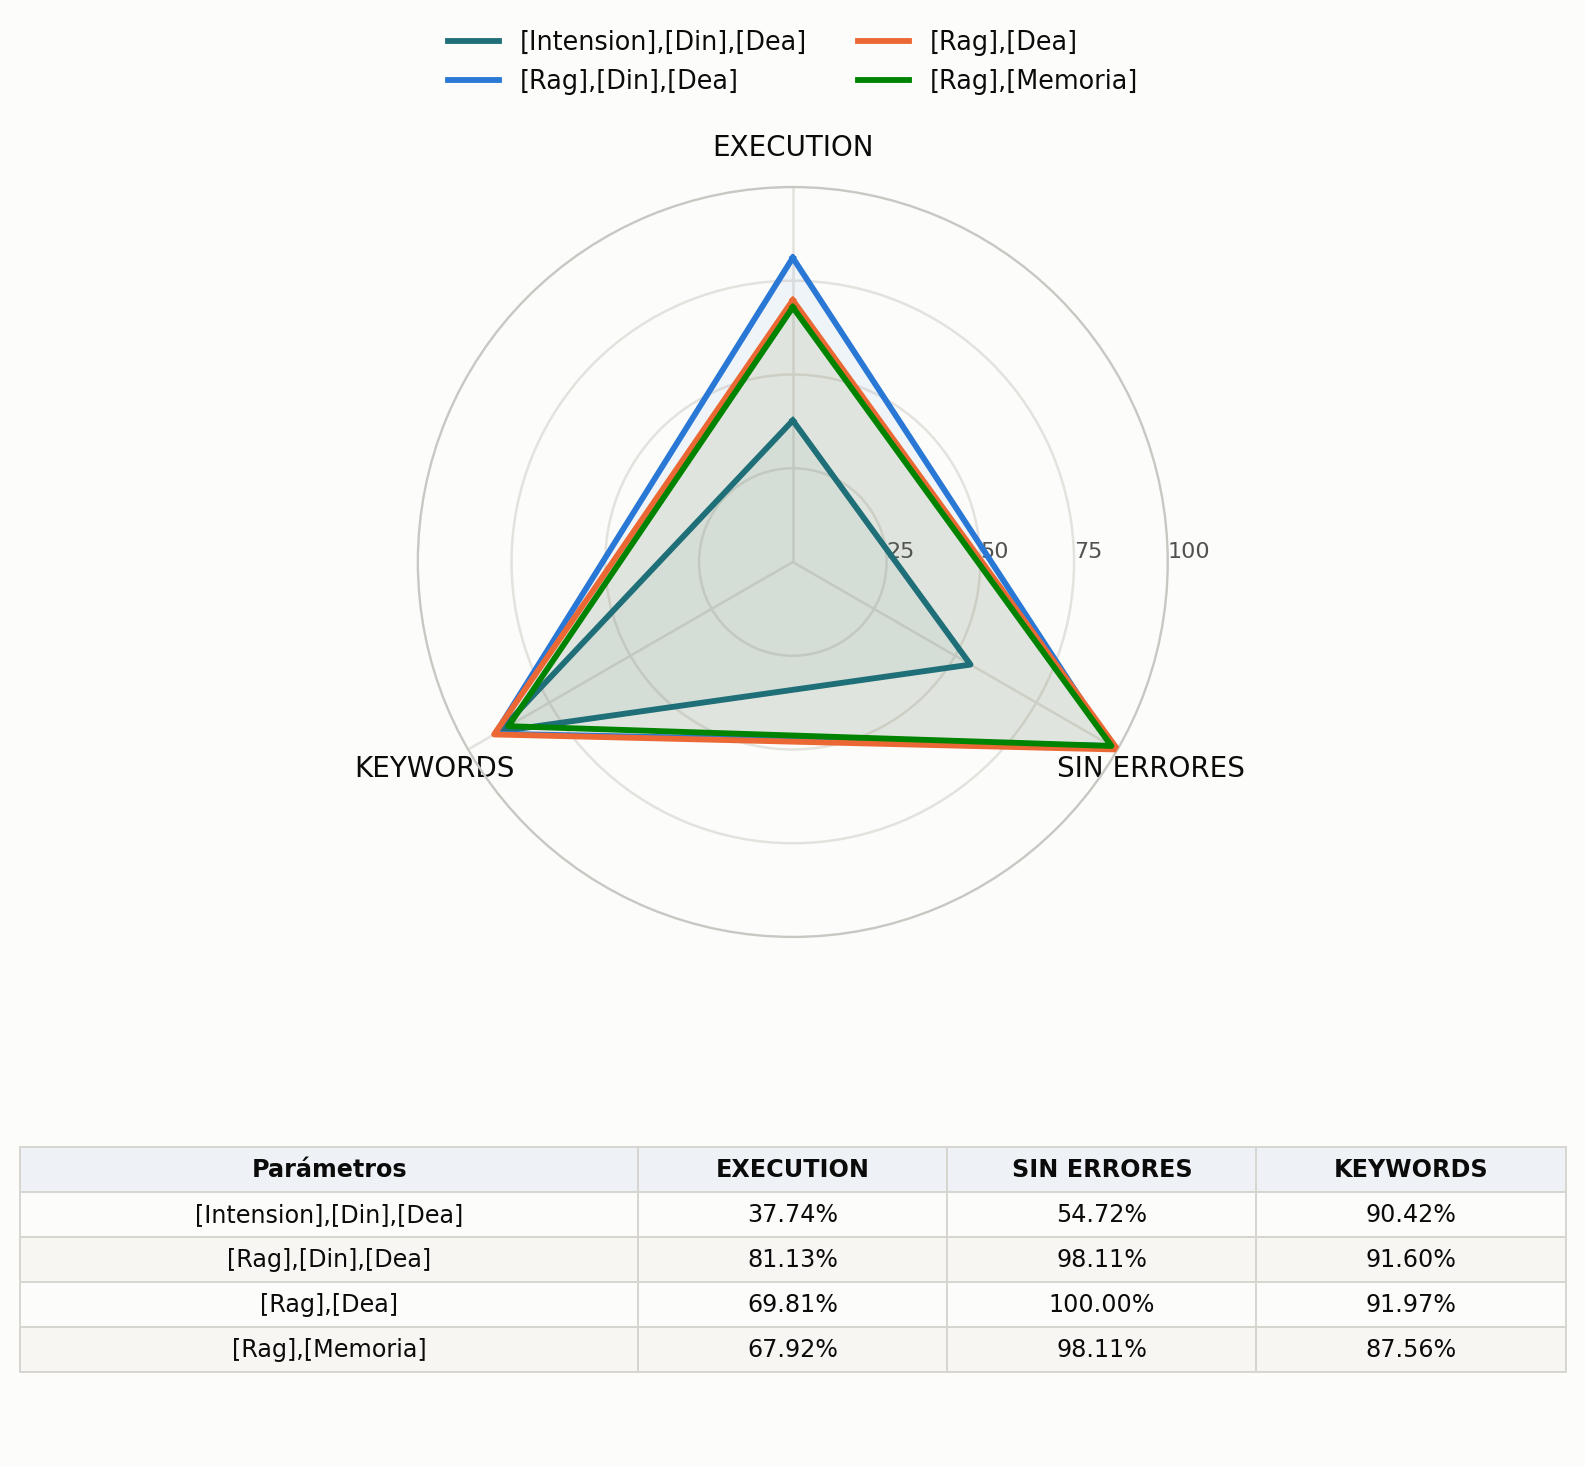
\includegraphics[width=0.9\linewidth]{Figura 5.3 - con autocorreccion.png}
	\caption{Robustez del sistema considerando mecanismos de autocorrección (SIN ERRORES). Las configuraciones que incorporan RAG alcanzan valores cercanos al 100\%, evidenciando alta robustez frente a errores sintácticos y referencias incorrectas mediante corrección iterativa.}
	\label{fig:sin_errores}
\end{figure}

No obstante, esta métrica debe interpretarse con cautela, ya que no distingue entre consultas correctamente generadas desde el primer intento y aquellas que requieren múltiples iteraciones de corrección. En este sentido, valores elevados de SIN ERRORES pueden reflejar una robustez operativa, pero no necesariamente una alta calidad inicial en la generación del SQL. La Figura~\ref{fig:sin_errores} muestra cómo las configuraciones con RAG logran alta robustez mediante mecanismos de corrección automática.

\subsection{Capacidad real de generación sin autocorrección (SIN\_AUTO\_CORRECCION)}

La métrica SIN\_AUTO\_CORRECCION permite evaluar de manera más estricta la capacidad del sistema para generar consultas SQL correctas desde el primer intento, sin depender de mecanismos de reparación automática. Esta métrica revela diferencias sustanciales entre configuraciones que, de otro modo, presentan valores similares en SIN ERRORES.

Los resultados muestran que configuraciones basadas únicamente en RAG o en modelado de Intensión dependen fuertemente de la autocorrección, alcanzando valores inferiores al 30\% en generación correcta inicial. Este comportamiento indica que, si bien dichas configuraciones pueden eventualmente producir consultas funcionales, lo hacen a costa de múltiples iteraciones de corrección.

En contraste, la configuración [RAG + DIN + DEA] alcanza un valor cercano al 89\% en SIN\_AUTO\_CORRECCION, lo que evidencia una alta capacidad de generación correcta directa. Este resultado sugiere que la combinación de recuperación contextual con descomposición y razonamiento orientado a la ejecución permite al sistema formular consultas más precisas desde el inicio, reduciendo la dependencia de ciclos de corrección posteriores.

\begin{figure}[htbp]
	\centering
	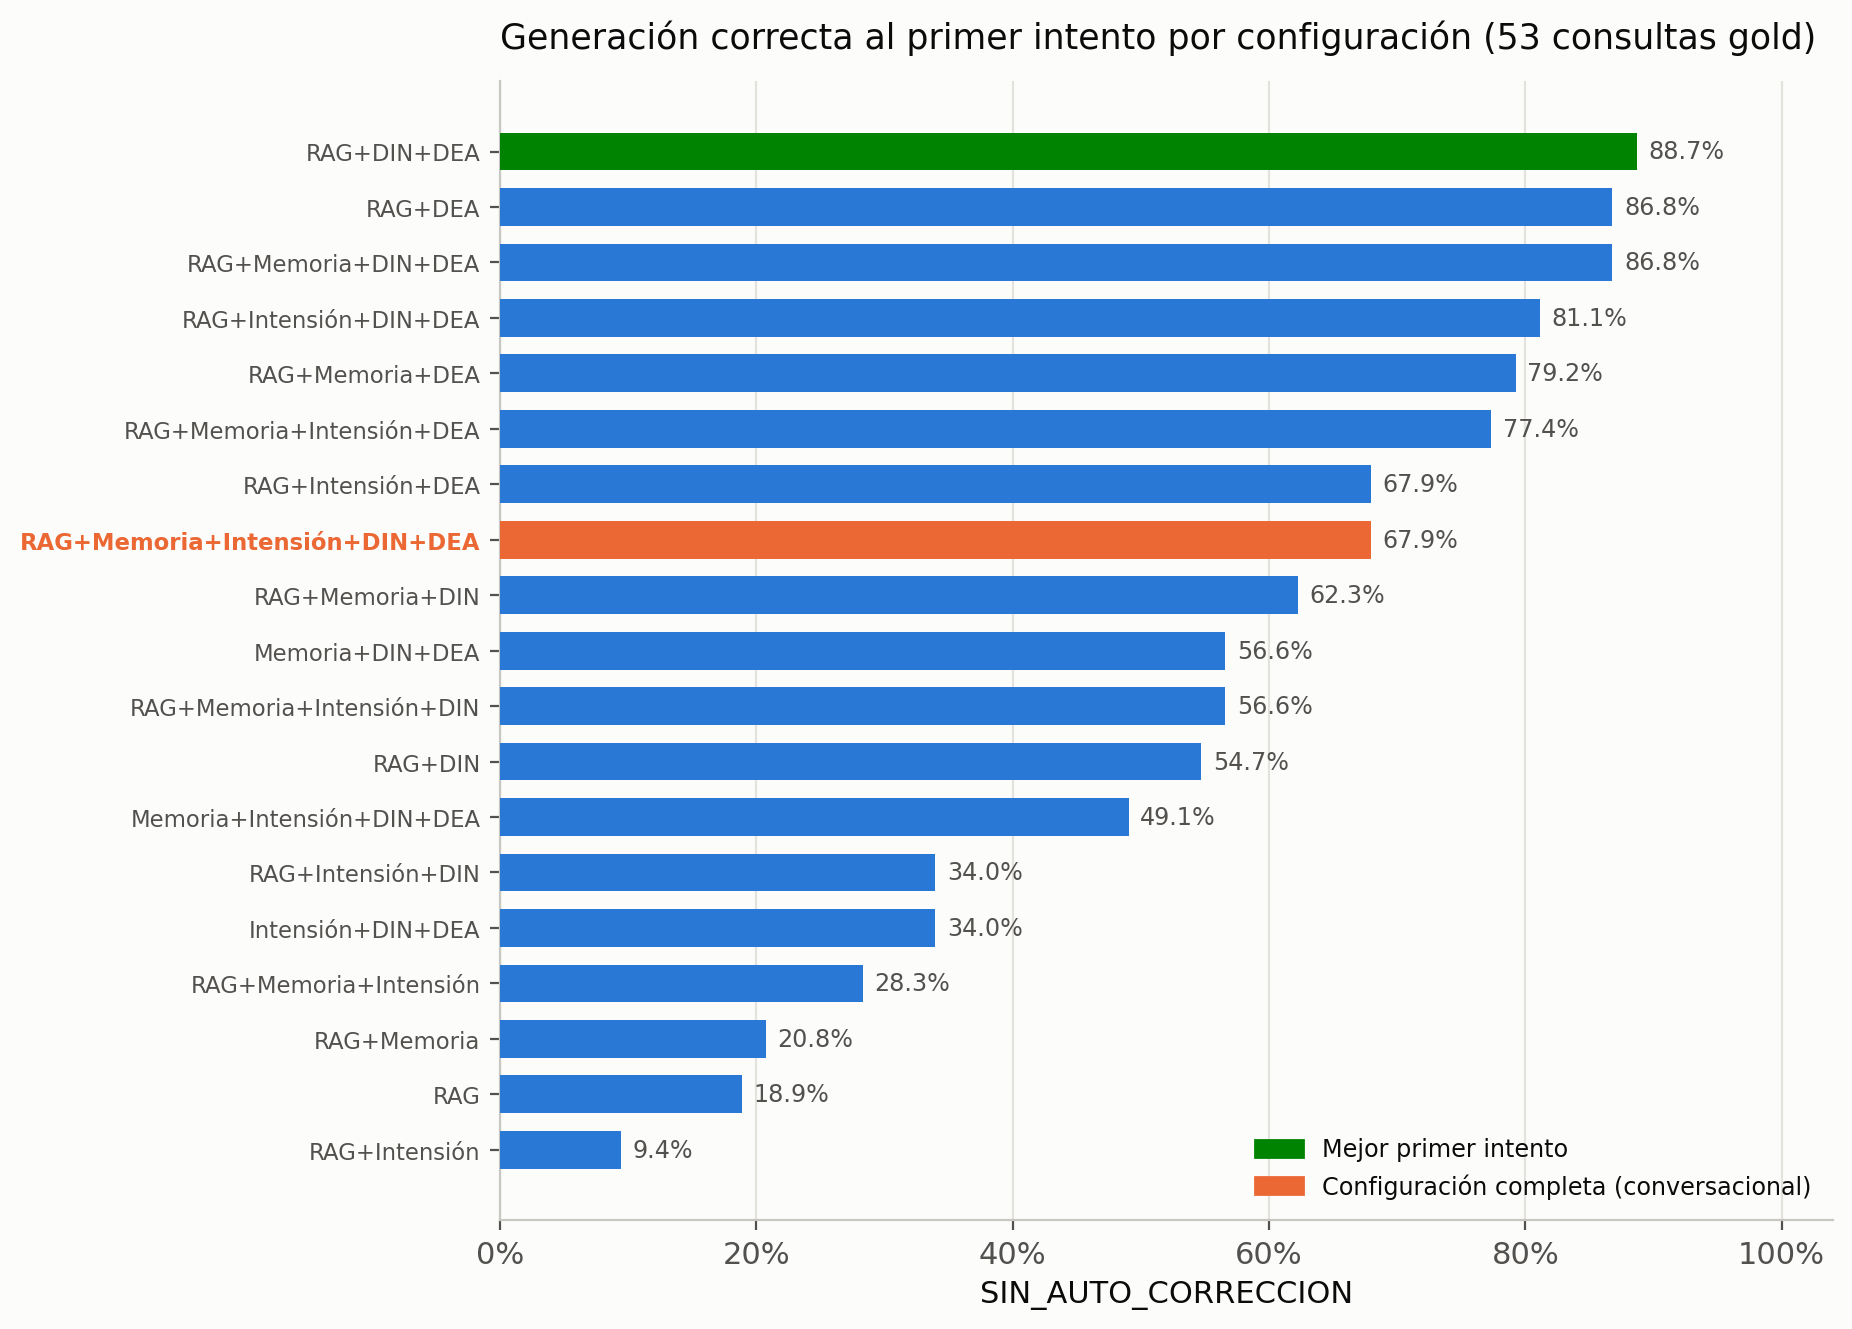
\includegraphics[width=\linewidth]{Figura 5.4 - Ranking SIN AUTO 19 configuraciones.png}
	\caption{Capacidad de generación sin autocorrección (SIN\_AUTO\_CORRECCION) para las 19 configuraciones evaluadas sobre las mismas 53 consultas gold. La configuración [RAG + DIN + DEA] lidera con 88,7\%, mientras que configuraciones basadas únicamente en RAG o Intensión dependen fuertemente de mecanismos de corrección iterativa; la configuración completa alcanza un 67,9\%, sacrificando parte de la generación directa a cambio de las capacidades conversacionales.}
	\label{fig:sin_autocorreccion}
\end{figure}

Esta métrica resulta clave para diferenciar entre robustez aparente y capacidad real de generación, especialmente en escenarios de producción donde la latencia y la previsibilidad del sistema son factores críticos. La Figura~\ref{fig:sin_autocorreccion} ilustra claramente las diferencias en la capacidad de generación directa entre las distintas configuraciones evaluadas.

\subsection{Validación de los módulos de Intensión y Memoria en escenarios conversacionales}

Además del análisis cuantitativo, se realizó una validación cualitativa orientada a evaluar el comportamiento de los módulos de Intensión y Memoria en escenarios conversacionales multi-turno, característicos de la interacción natural entre usuarios y sistemas ERP.

En sistemas de transformación de lenguaje natural a SQL orientados a la interacción conversacional, no todas las entradas del usuario constituyen solicitudes ejecutables. Expresiones iniciales como saludos, preguntas genéricas o referencias incompletas carecen de la información semántica necesaria para generar una consulta válida. En este contexto, la ejecución inmediata de una consulta SQL no solo resulta innecesaria, sino potencialmente incorrecta.

Para abordar este problema, el sistema incorpora un módulo de Intensión, cuya función principal es determinar si una entrada del usuario contiene información suficiente para ser interpretada como una solicitud ejecutable. Este módulo actúa como una capa de validación semántica previa a la generación de SQL, evitando intentos de ejecución cuando la intención del usuario es ambigua, incompleta o puramente conversacional.

No obstante, en escenarios reales de interacción humano-sistema, la información requerida para ejecutar una consulta puede encontrarse distribuida a lo largo de múltiples turnos de diálogo. En estos casos, el módulo de Memoria desempeña un rol complementario, permitiendo conservar y recuperar el contexto semántico generado en interacciones previas. La combinación de ambos módulos habilita la reconstrucción de solicitudes completas a partir de fragmentos conversacionales, sin exigir que el usuario formule explícitamente una consulta totalmente especificada en un único mensaje.

\subsubsection{Ejemplo ilustrativo de escenario multi-turno}

Para ilustrar el funcionamiento coordinado de ambos módulos, se presenta el siguiente caso de uso representativo:

\textbf{Turno 1 -- Usuario:} ``Hola, ¿me puedes ayudar con los productos?''

\begin{itemize}
	\item \textit{Intensión detectada:} No ejecutable
	\item \textit{Acción del sistema:} No se genera SQL
\end{itemize}

En este primer turno, el módulo de Intensión determina que la entrada no corresponde a una solicitud ejecutable, dado que no se especifica ninguna acción concreta ni criterios de selección. En consecuencia, el sistema no genera ni ejecuta una consulta SQL, evitando así una interpretación errónea de la intención del usuario.

\textbf{Turno 2 -- Usuario:} ``Dame el nombre de los primeros 5''

\begin{itemize}
	\item \textit{Memoria recupera el contexto:} productos
	\item \textit{Intensión detectada:} Ejecutable
	\item \textit{Consulta implícita reconstruida:} ``Obtener el nombre de los primeros 5 productos''
	\item \textit{Acción del sistema:} Generación y ejecución del SQL
\end{itemize}

En este segundo turno, el módulo de Memoria recupera el contexto semántico previamente mencionado (productos). Con esta información, el módulo de Intensión evalúa que la combinación de ambos turnos constituye una solicitud completa y ejecutable. El sistema puede entonces reconstruir implícitamente la consulta como ``Obtener el nombre de los primeros cinco productos'' y proceder a la generación y ejecución del SQL correspondiente.

Este mecanismo permite prevenir ejecuciones inválidas o ambiguas, al tiempo que soporta interacciones progresivas y naturales, donde el usuario no necesita formular una consulta completa en un único turno. De esta forma, los módulos de Intensión y Memoria no deben evaluarse exclusivamente por métricas de ejecución, sino por su capacidad de regular cuándo es semánticamente válido ejecutar una consulta, contribuyendo a la confiabilidad global del sistema en escenarios conversacionales reales.

\subsection{Medición del costo computacional y consumo de tokens}

Como parte del proceso de evaluación experimental, se registró el consumo real de tokens y el costo asociado a la generación de consultas SQL para todas las configuraciones evaluadas. Este análisis tiene como objetivo cuantificar el impacto económico de ejecutar un estudio de ablación completo en un sistema NL-to-SQL basado en modelos de lenguaje de gran escala.

En total, la ejecución de todas las combinaciones experimentales dio lugar a 1.007 solicitudes de generación de SQL, considerando tanto intentos iniciales como ajustes derivados de mecanismos de autocorrección. Estas solicitudes se procesaron utilizando distintos modelos de lenguaje con capacidades diferenciadas, seleccionados dinámicamente según el tipo de tarea (generación inicial, razonamiento, verificación o corrección).

El costo total acumulado de estas ejecuciones fue de \$34.777 pesos colombianos (COP), correspondiente a la generación y procesamiento de tokens de entrada y salida durante el periodo experimental.

\subsubsection{Distribución del consumo de tokens}

El consumo total de tokens se distribuyó entre tokens de entrada (input tokens), tokens de salida (output tokens) y tokens reutilizados mediante mecanismos de caché. La mayor parte del consumo corresponde a tokens de entrada, lo cual es consistente con la naturaleza del problema, dado que las solicitudes incluyen contexto estructural, esquemas de base de datos y fragmentos conversacionales acumulados.

De forma resumida, el experimento utilizó aproximadamente:

\begin{itemize}
	\item Más de 25 millones de tokens de entrada, considerando modelos de distintas capacidades.
	\item Cerca de 2,8 millones de tokens de salida, asociados a la generación de consultas SQL y respuestas intermedias.
	\item Una fracción menor de tokens cacheados, con un impacto económico marginal.
\end{itemize}

Este patrón confirma que los costos del sistema están dominados por la cantidad y longitud del contexto proporcionado al modelo, más que por la longitud de las respuestas generadas.

\begin{figure}[htbp]
	\centering
	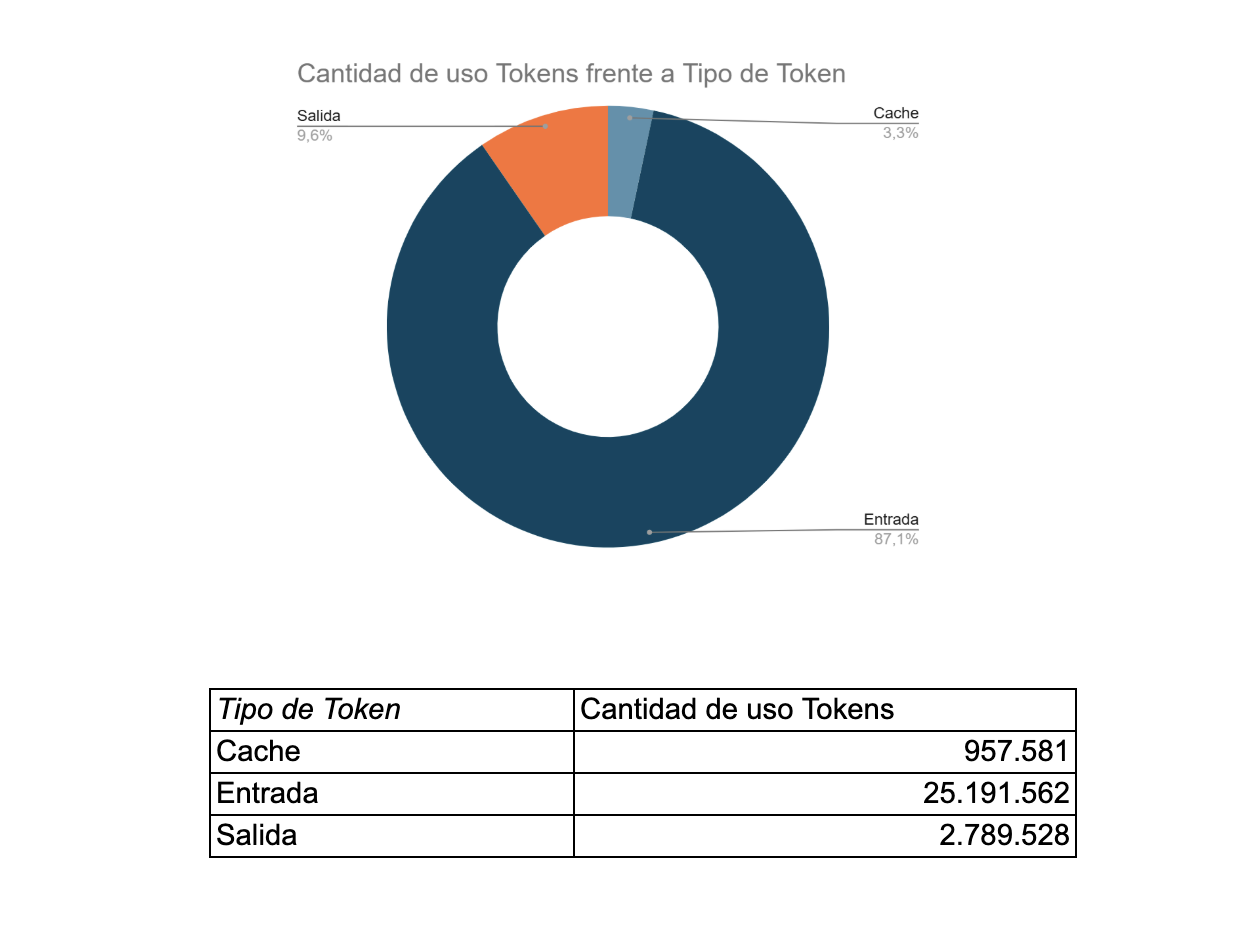
\includegraphics[width=\linewidth]{Figura 5.5 - Catidad de Tockens.png}
	\caption{Distribución del consumo de tokens durante la evaluación experimental. Se observa que los tokens de entrada dominan el consumo total, reflejando la naturaleza intensiva en contexto del sistema Text-to-SQL propuesto.}
	\label{fig:cantidad_tokens}
\end{figure}

\begin{figure}[htbp]
	\centering
	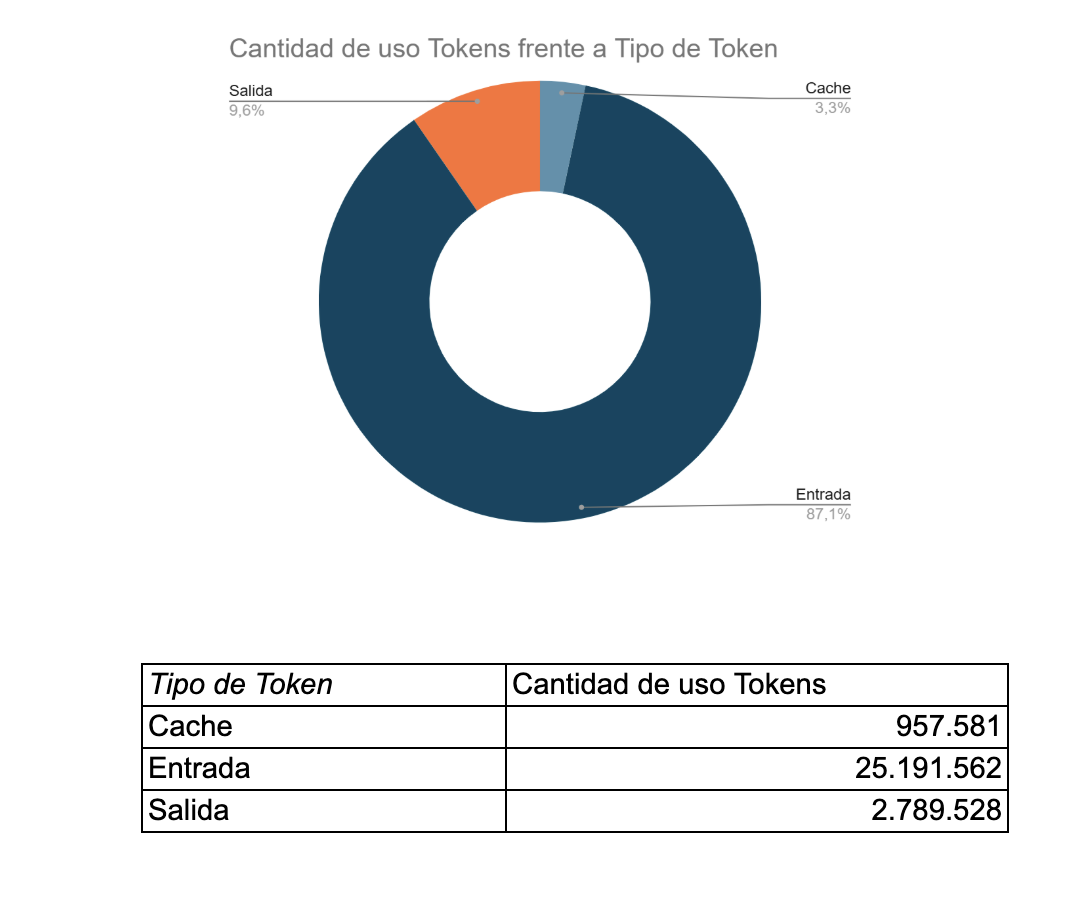
\includegraphics[width=\linewidth]{Figura 5.6 - Cantidad de uso.png}
	\caption{Distribución del uso de modelos de lenguaje durante el experimento. Se evidencia la selección dinámica de modelos según el tipo de tarea, optimizando el balance entre capacidad y costo computacional.}
	\label{fig:cantidad_uso}
\end{figure}

\subsubsection{Costo promedio por solicitud}

Considerando el total de 1.007 solicitudes SQL, el costo promedio por solicitud se estima en aproximadamente:

\begin{center}
	\textbf{\$34,5 COP por solicitud SQL}
\end{center}

Este valor incluye tanto solicitudes exitosas en el primer intento como aquellas que requirieron procesos de autocorrección. Desde una perspectiva práctica, este resultado indica que la evaluación exhaustiva de múltiples arquitecturas puede realizarse con un costo económico reducido, incluso al emplear modelos de lenguaje avanzados.

\subsubsection{Impacto del diseño arquitectónico en el costo}

Si bien este análisis no persigue la optimización económica como objetivo principal, los resultados sugieren que arquitecturas más robustas, como [RAG + DIN + DEA], reducen indirectamente el costo computacional al disminuir la necesidad de reintentos y autocorrecciones. En contraste, configuraciones con baja capacidad de generación correcta inicial tienden a incrementar el número de solicitudes necesarias para obtener una consulta válida.

Este hallazgo refuerza la idea de que mejorar la calidad de la generación en el primer intento no solo impacta la exactitud del sistema, sino también su eficiencia operativa y su costo total de uso.

\subsubsection{Consideraciones sobre reproducibilidad y validez}

Los costos reportados corresponden a un entorno experimental específico y a un conjunto fijo de preguntas. No obstante, al tratarse de métricas directamente derivadas del consumo de tokens, estos resultados ofrecen una referencia concreta y reproducible para evaluar la viabilidad económica de sistemas NL-to-SQL en escenarios reales.

Este análisis complementa las métricas de precisión y ejecución presentadas anteriormente, aportando una dimensión práctica que resulta especialmente relevante para la adopción de este tipo de sistemas en entornos productivos.

\subsection{Análisis del Time To Answer (TTA) en el workflow multi-agente}

El Time To Answer (TTA) mide el tiempo total transcurrido desde que el usuario emite una consulta en lenguaje natural hasta que el workflow multi-agente finaliza completamente su ejecución y retorna una respuesta definitiva. A diferencia de métricas de latencia asociadas a una única inferencia, el TTA captura de forma integral el costo temporal real del sistema, incluyendo todas las inferencias internas y ciclos de razonamiento necesarios para producir una consulta SQL válida y ejecutable.

En particular, el TTA incorpora el tiempo asociado a la detección y validación de intención, la recuperación de contexto mediante mecanismos de Retrieval-Augmented Generation (RAG), el razonamiento estructural, la generación inicial del SQL y, cuando aplica, los ciclos iterativos de autocorrección. Por tanto, esta métrica refleja de manera más fiel la experiencia del usuario final y el costo computacional total del razonamiento distribuido entre agentes, aspecto crítico en entornos empresariales como los sistemas ERP.

\subsubsection{Resultados agregados de TTA por configuración}

La Tabla 5.7 resume los valores promedio, mínimo y máximo de TTA para las distintas configuraciones arquitectónicas evaluadas, junto con sus métricas de desempeño en Execution Accuracy, SIN ERRORES y SIN\_AUTO\_CORRECCION. Los resultados evidencian una variabilidad considerable entre configuraciones, tanto en términos de latencia promedio como de dispersión extrema.

De forma general, los valores de TTA promedio oscilan entre aproximadamente 10 y 30 segundos. No obstante, algunas configuraciones presentan tiempos máximos superiores a los 100 segundos, lo que indica la presencia de ejecuciones particularmente costosas desde el punto de vista temporal.

\begin{table}[htbp]
	\centering
	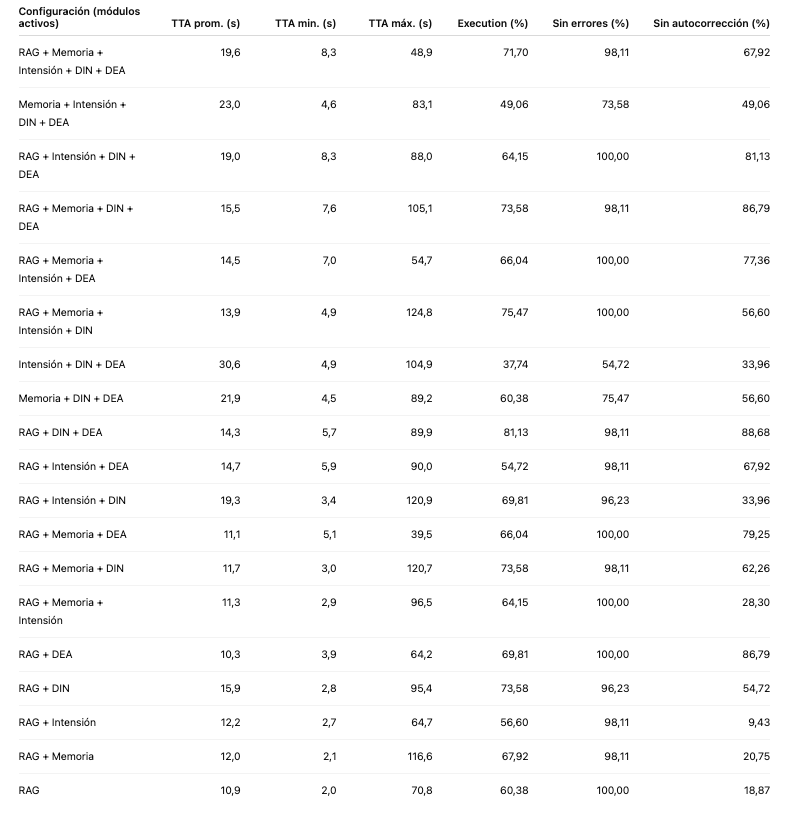
\includegraphics[width=0.95\linewidth]{Tabla 4 Time To Answer.png}
	\caption{Resultados de Time To Answer (TTA) por configuración arquitectónica}
	\label{tab:tta_results}
	\tablefont
	\textit{Nota.} El Time To Answer (TTA) se mide en segundos (s). Execution corresponde a Execution Accuracy. Sin errores representa la robustez del workflow considerando la ejecución con mecanismos de corrección activados. Sin autocorrección mide la proporción de consultas SQL correctas generadas desde el primer intento, sin requerir ciclos adicionales de corrección.
\end{table}

\subsubsection{Distribución y variabilidad del TTA}

El análisis de la distribución del TTA muestra que la variabilidad no está directamente asociada al número de módulos activos en la arquitectura, sino al número de iteraciones internas requeridas para converger hacia una consulta válida. En particular, las configuraciones con bajo desempeño en SIN\_AUTO\_CORRECCION exhiben valores más elevados tanto en el TTA promedio como en el TTA máximo.

Este comportamiento sugiere que cada fallo en la generación inicial del SQL introduce ciclos adicionales de razonamiento, validación y corrección, incrementando de forma acumulativa el tiempo total de respuesta. En consecuencia, el TTA se ve fuertemente influenciado por la capacidad del sistema de producir una consulta correcta desde el primer intento.

\begin{figure}[htbp]
	\centering
	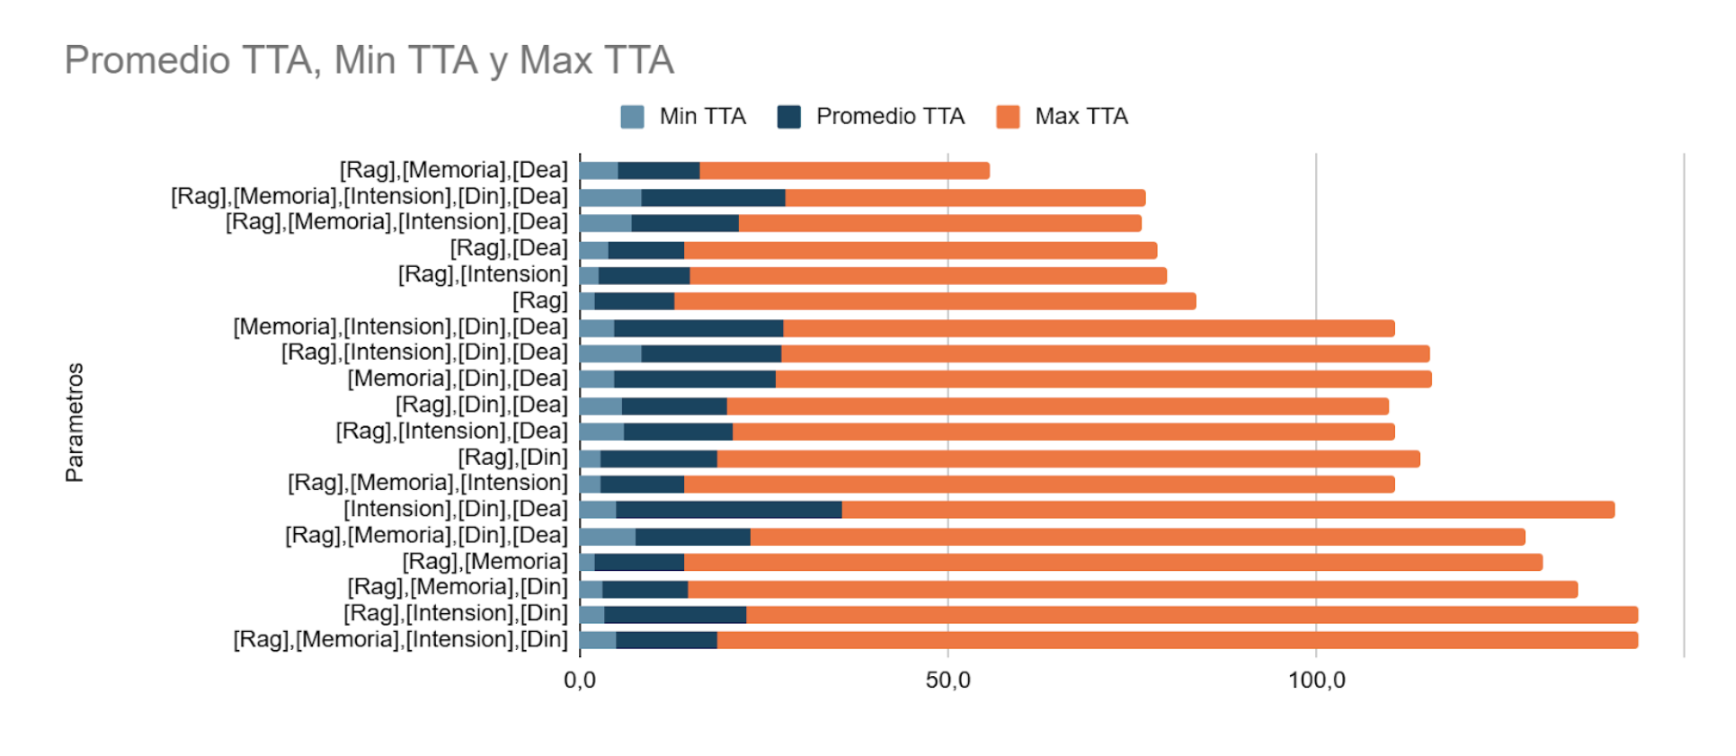
\includegraphics[width=\linewidth]{Figura 5.7 Distribución del TTA.png}
	\caption{Distribución del Time To Answer (TTA) por configuración arquitectónica. Se observa la variabilidad en los tiempos de respuesta, evidenciando que las configuraciones con menor capacidad de generación correcta inicial presentan mayor dispersión y valores extremos más elevados.}
	\label{fig:distribucion_tta}
\end{figure}

\subsubsection{Configuraciones sin grounding contextual}

La configuración compuesta únicamente por Intension + Din + Dea presenta el mayor TTA promedio (30,6 s), así como uno de los valores máximos más elevados. Este comportamiento se corresponde con su bajo desempeño en Execution Accuracy (37,74\%) y SIN\_AUTO\_CORRECCION (33,96\%).

Estos resultados evidencian que, en ausencia de grounding contextual, el workflow multi-agente incurre en múltiples intentos fallidos antes de producir una respuesta aceptable. El incremento del TTA no refleja un razonamiento más profundo o efectivo, sino una ineficiencia derivada de errores recurrentes durante la generación y validación del SQL.

Este escenario constituye un contraejemplo empírico relevante: el razonamiento estructural, cuando no está correctamente contextualizado, puede incrementar significativamente el tiempo total de resolución sin mejorar la calidad del resultado final.

\subsubsection{Impacto del grounding mediante RAG sobre el TTA}

Las configuraciones que incorporan RAG muestran una reducción consistente del TTA promedio, incluso cuando incluyen múltiples módulos adicionales. Por ejemplo, la configuración Rag + Din + Dea alcanza un TTA promedio de 14,3 s, al mismo tiempo que obtiene el mejor desempeño en Execution Accuracy (81,13\%) y SIN\_AUTO\_CORRECCION (88,68\%).

Este comportamiento indica que el grounding proporcionado por RAG permite al workflow converger más rápidamente hacia una solución válida, reduciendo la necesidad de ciclos iterativos de razonamiento y autocorrección. En consecuencia, RAG no solo mejora la exactitud del sistema, sino que también optimiza su eficiencia temporal a nivel del workflow completo.

\begin{figure}[htbp]
	\centering
	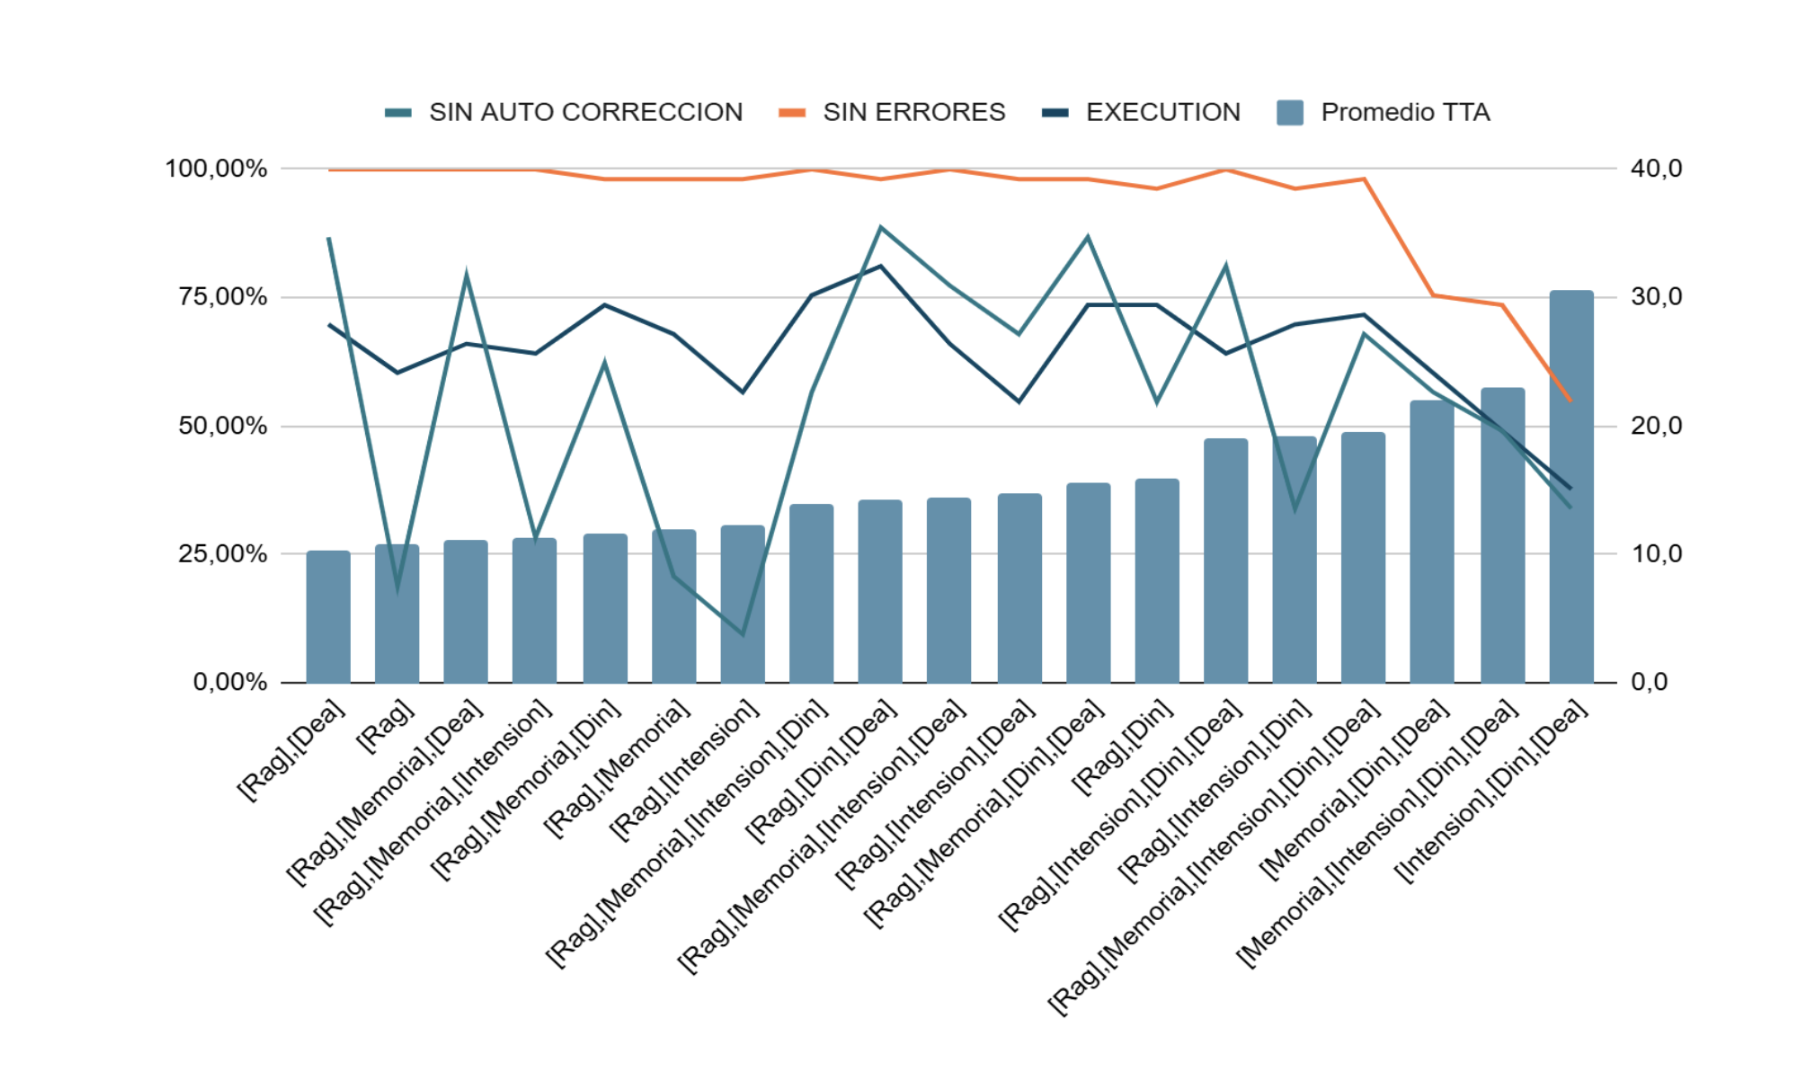
\includegraphics[width=\linewidth]{Figura 5.8 Relacion RAG.png}
	\caption{Relación entre la incorporación de RAG y el Time To Answer. Las configuraciones que incluyen RAG muestran una reducción consistente del TTA promedio, demostrando que el grounding contextual no solo mejora la exactitud sino también la eficiencia temporal del sistema.}
	\label{fig:relacion_rag}
\end{figure}

\subsubsection{Relación entre SIN\_AUTO\_CORRECCION y TTA}

Considerando el conjunto completo de configuraciones, la correlación lineal entre SIN\_AUTO\_CORRECCION y TTA promedio es débil ($r \approx -0{,}05$): la generación correcta al primer intento no es, por sí sola, el factor que gobierna el tiempo de respuesta. El patrón dominante es otro: la configuración sin grounding contextual, Intensión + DIN + DEA, concentra a la vez el mayor TTA promedio (30,6 s) y el menor SIN\_AUTO\_CORRECCION (33,96\%), mientras que entre las configuraciones con RAG el TTA permanece comprimido en la franja de 10 a 16 segundos con relativa independencia de su generación inicial —incluso las de SIN\_AUTO\_CORRECCION inferior al 25\% (RAG, RAG + Intensión, RAG + Memoria) resuelven en torno a 11--12 s, porque el grounding permite converger sin acumular ciclos de corrección costosos.

Así, la relación entre calidad inicial y tiempo se manifiesta solo cuando el error de generación coincide con la ausencia de grounding: entonces cada intento fallido añade ciclos de inferencia y validación que disparan el TTA. Cuando el sistema dispone de RAG, la recuperación del esquema absorbe ese costo. El factor determinante del desempeño temporal no es, por tanto, el SIN\_AUTO\_CORRECCION aislado, sino la presencia de grounding contextual (Figura~\ref{fig:relacion_rag}).

\begin{figure}[htbp]
	\centering
	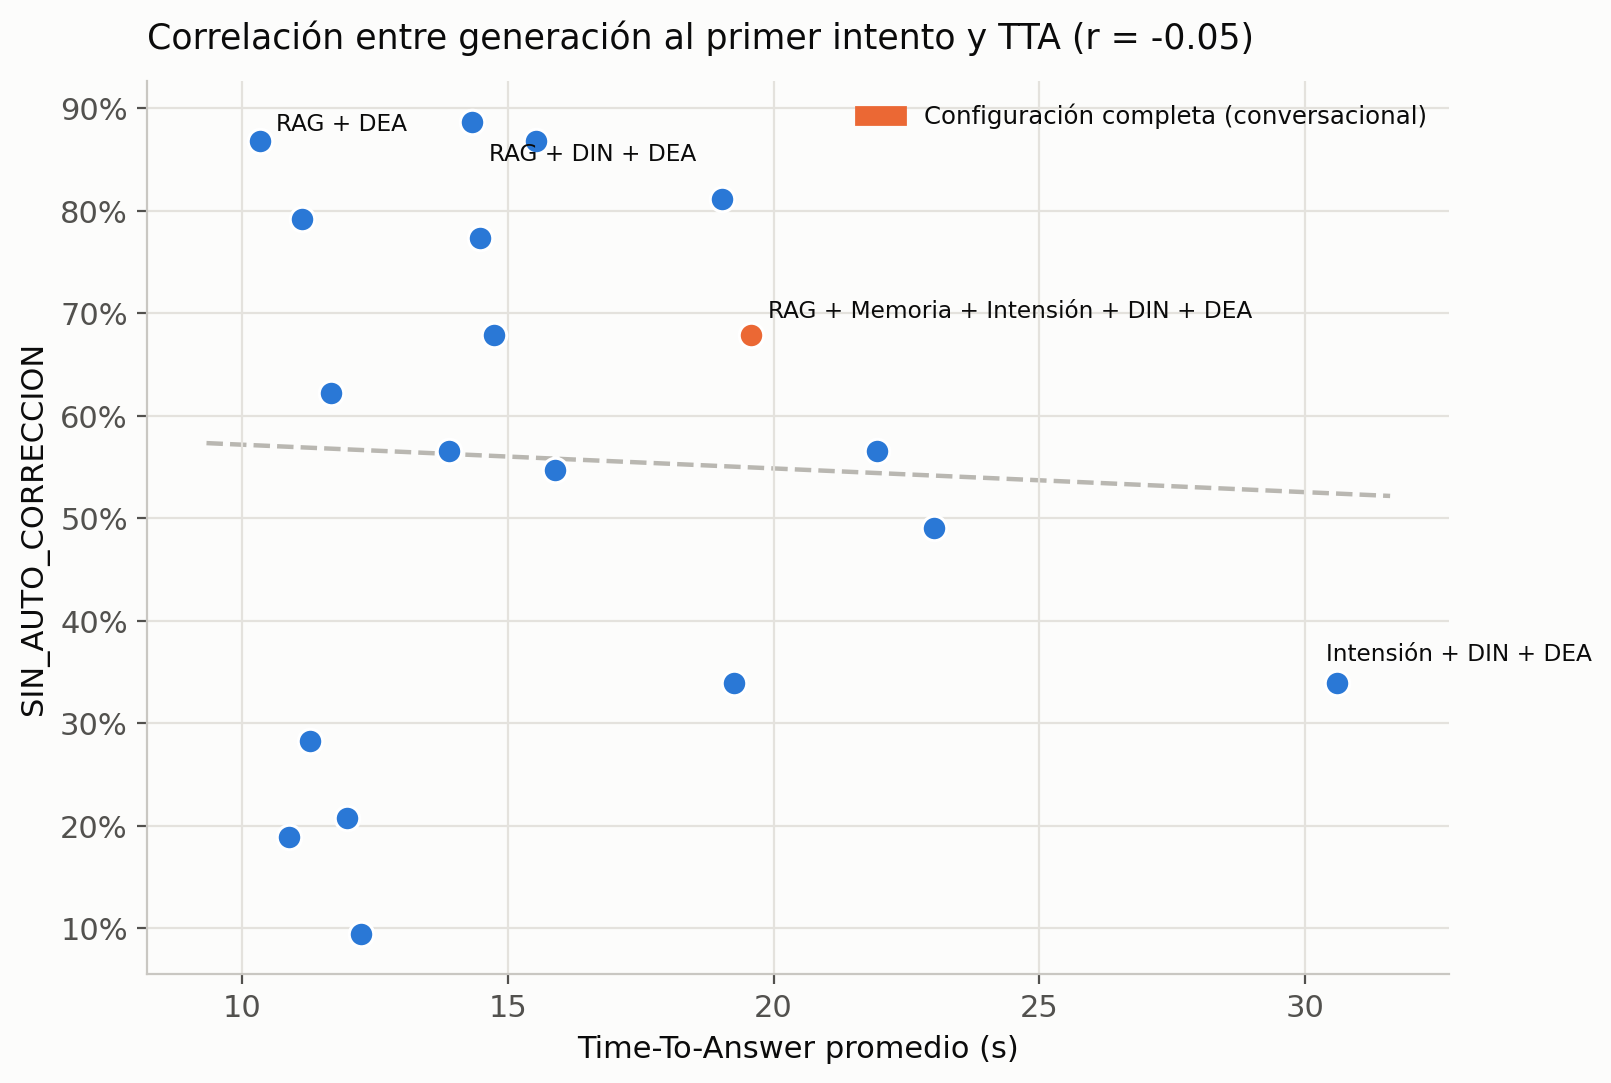
\includegraphics[width=\linewidth]{Figura 5.9 Correlacion sin AC.png}
	\caption{Relación entre SIN\_AUTO\_CORRECCION y Time To Answer promedio para las 19 configuraciones evaluadas. La correlación lineal es débil ($r \approx -0{,}05$): el mayor TTA no lo determina la generación inicial por sí sola, sino la ausencia de grounding contextual (configuración sin RAG en el extremo superior derecho). Entre las configuraciones con RAG el TTA permanece comprimido en 10--16 s con independencia de su generación al primer intento.}
	\label{fig:correlacion_sin_ac}
\end{figure}

\subsubsection{Rol de Memoria e Intensión en el TTA}

Las configuraciones que incorporan los módulos de Memoria e Intensión presentan un comportamiento diferenciado en términos de TTA. En escenarios conversacionales multi-turno, estos módulos permiten evitar ejecuciones prematuras y reconstruir consultas completas a partir de fragmentos distribuidos en varios mensajes, mejorando la coherencia semántica del sistema.

No obstante, cuando la generación inicial del SQL no es suficientemente robusta, la acumulación de contexto y la validación adicional pueden incrementar el TTA máximo, como se observa en algunas configuraciones con valores elevados de TTA extremo. Este fenómeno no debe interpretarse como una deficiencia del sistema, sino como una consecuencia directa del soporte a interacciones conversacionales más complejas y naturales.

\subsubsection{Configuración con mejor compromiso entre calidad y tiempo}

Entre todas las configuraciones evaluadas, Rag + Din + Dea presenta el mejor equilibrio global entre exactitud, robustez y eficiencia temporal. Esta arquitectura combina:

\begin{itemize}
	\item Un TTA promedio bajo (14,3 s)
	\item Alta Execution Accuracy (81,13\%)
	\item Elevada generación correcta sin autocorrección (88,68\%)
\end{itemize}

Estos resultados demuestran que un workflow multi-agente correctamente balanceado no solo mejora la calidad de las respuestas, sino que también reduce el tiempo total requerido para completarlas, al minimizar la necesidad de razonamiento iterativo.

\subsubsection{Implicaciones para sistemas NL-to-SQL multi-agente}

El análisis del TTA confirma que la eficiencia temporal de un sistema NL-to-SQL multi-agente está fuertemente influenciada por su capacidad de generar consultas correctas desde el primer intento. Arquitecturas frágiles no solo presentan menores tasas de ejecución correcta, sino que también incrementan significativamente el tiempo total de respuesta, afectando negativamente la experiencia del usuario y el costo computacional.

En consecuencia, el diseño de sistemas NL-to-SQL multi-agente debe priorizar el grounding contextual y el razonamiento estructural efectivo, no solo como mecanismos de mejora de exactitud, sino como factores clave para garantizar un comportamiento eficiente y escalable a nivel de workflow completo.

\subsection{Medición del Context Retention Rate (CRR)}
\label{sec:crr_dialogo}

El Context Retention Rate (CRR) evalúa la capacidad del sistema para retener, recuperar y reutilizar correctamente el contexto relevante a lo largo de interacciones conversacionales multi-turno. A diferencia de métricas centradas en consultas aisladas, CRR mide el comportamiento del sistema cuando las solicitudes del usuario dependen parcial o totalmente de información introducida en turnos previos, como referencias elípticas, anafóricas o implícitas.

Para esta evaluación, el CRR se midió sobre el conjunto conversacional multi-turno completo descrito en la Sección~\ref{sec:datasets}, ejecutando el flujo agentivo real contra la base de datos de prueba. De los 759 turnos de las 100 conversaciones, \textbf{313 corresponden a seguimientos dependientes de memoria} (referencias elípticas, anafóricas o implícitas del tipo ``ahora lo mismo pero con\ldots'', ``los primeros 5'', ``ahora con Cuba''), que solo pueden resolverse recuperando la entidad, los campos o los filtros establecidos en turnos previos. La Figura~\ref{fig:crr_evaluation} presenta el CRR desagregado por tipo de seguimiento contextual.

\begin{figure}[htbp]
	\centering
	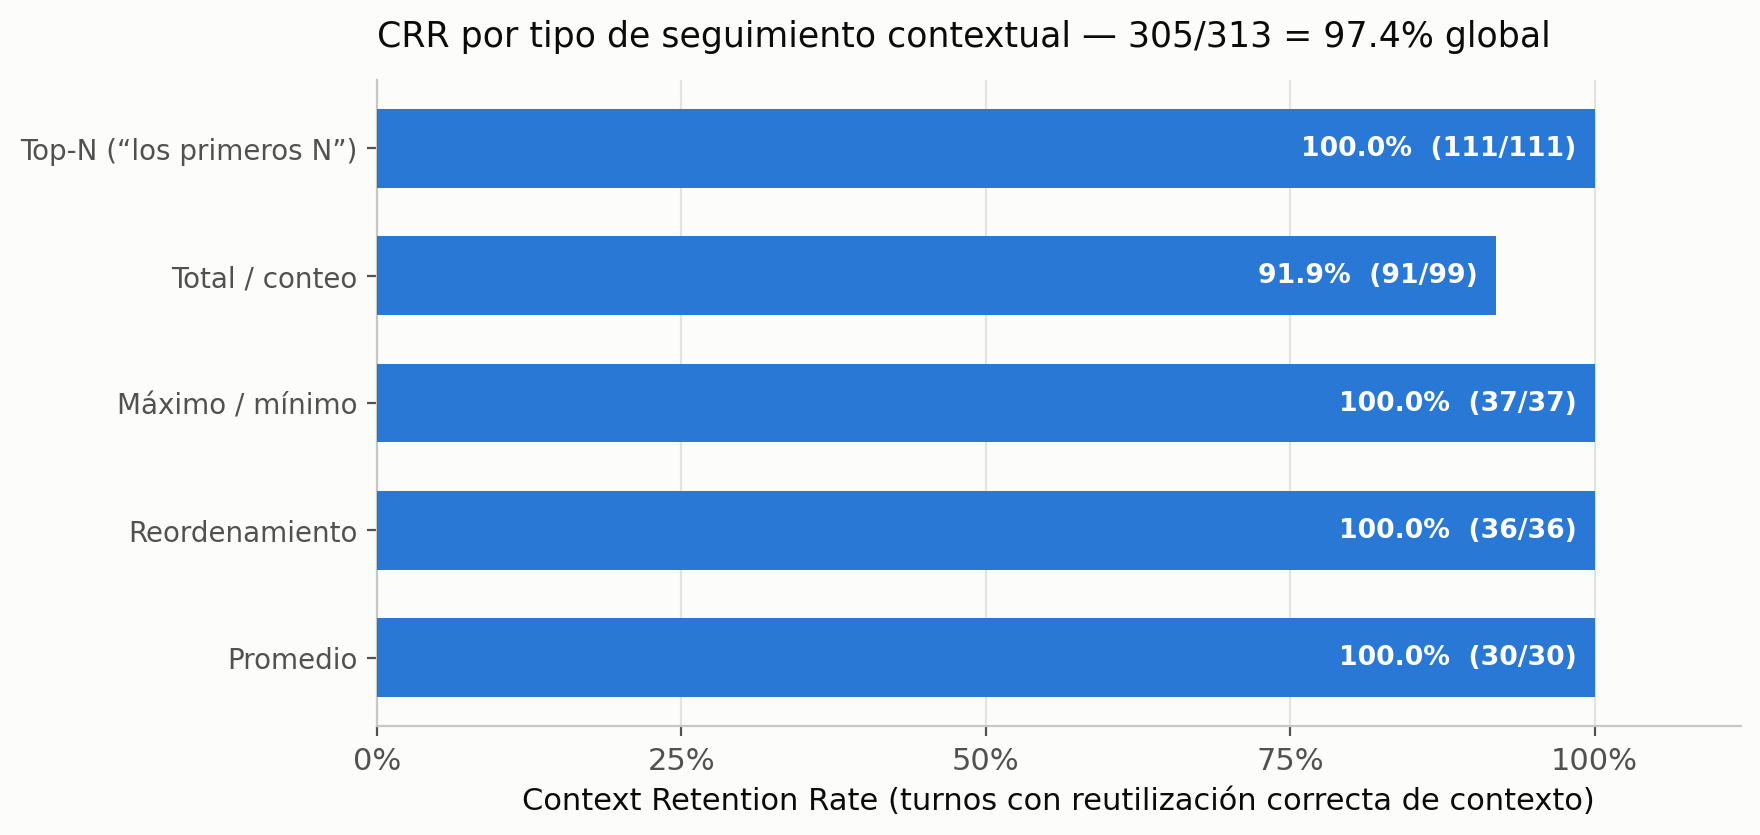
\includegraphics[width=0.8\linewidth]{Figura - Evaluacion de CRR.png}
	\caption{Context Retention Rate (CRR) sobre los 313 turnos de seguimiento dependientes de memoria del conjunto conversacional, desagregado por tipo de referencia contextual. El sistema reutilizó correctamente el contexto en el 97,4\% de los casos (305/313); las únicas fallas se concentran en seguimientos de tipo total/conteo.}
	\label{fig:crr_evaluation}
	\tablefont
	\textit{Nota.} Un turno se cuenta como acierto (CRR\_hit) cuando el sistema reconoce la referencia elíptica y reconstruye la solicitud a partir del contexto previo, en lugar de tratar el mensaje como una petición aislada o pedir que el usuario repita la información.
\end{figure}

\subsubsection{Definición y cálculo del CRR}

Un turno se clasifica como \textit{context-dependent} cuando la solicitud del usuario no es completamente ejecutable de forma autónoma, y requiere información semántica previa (por ejemplo, entidad, campos, filtros o límites definidos anteriormente). Un turno se considera exitoso (CRR\_hit = Sí) si el sistema:

\begin{itemize}
	\item Recupera correctamente el contexto relevante de turnos previos, y
	\item Lo aplica de forma consistente en la consulta SQL generada, sin requerir que el usuario repita explícitamente la información.
\end{itemize}

De los 313 turnos dependientes de memoria, el sistema reconstruyó correctamente la solicitud a partir del contexto previo en 305, lo que arroja el CRR global del sistema:

\begin{equation}
	\text{CRR} = \frac{\text{Turnos con CRR\_hit}}{\text{Turnos context-dependent}} = \frac{305}{313} = 0{,}974 \; (97{,}4\%)
\end{equation}

El desglose por tipo de referencia (Figura~\ref{fig:crr_evaluation}) muestra retención perfecta en los seguimientos que reutilizan una entidad para reproyectarla, reordenarla, limitarla o calcular un extremo, y concentra las ocho únicas fallas en los de tipo total/conteo (91/99), donde reconstruir el agregado desde el contexto es más ambiguo. El diálogo controlado de once turnos del escenario base (Sección~\ref{sec:crr_dialogo}) reproduce este comportamiento a pequeña escala: sus cuatro turnos dependientes de contexto (3, 6, 7 y 11) se resolvieron correctamente ($4/4 = 100\%$).

No obstante, retener el contexto y \emph{ejecutar la consulta exacta} son cosas distintas. La Figura~\ref{fig:contexto_mt} contrasta la calidad del SQL entre los turnos iniciales (que parten de una pregunta autónoma) y los turnos de seguimiento (que deben reconstruirse desde la memoria). En los turnos iniciales, la Execution Accuracy alcanza el 88,0\%; en los seguimientos contextuales desciende al 62,9\%. Esta brecha es esperable y semánticamente informativa: reconstruir una consulta a partir de fragmentos conversacionales previos es intrínsecamente más difícil que traducir una pregunta completa, ya que exige inferir correctamente qué entidad, campos y filtros deben heredarse del contexto. Aun así, cerca de dos de cada tres seguimientos producen resultados idénticos a los de la consulta de referencia, lo que confirma que el módulo de Memoria aporta una capacidad real —no meramente ilustrativa— de resolución contextual.

\begin{figure}[htbp]
	\centering
	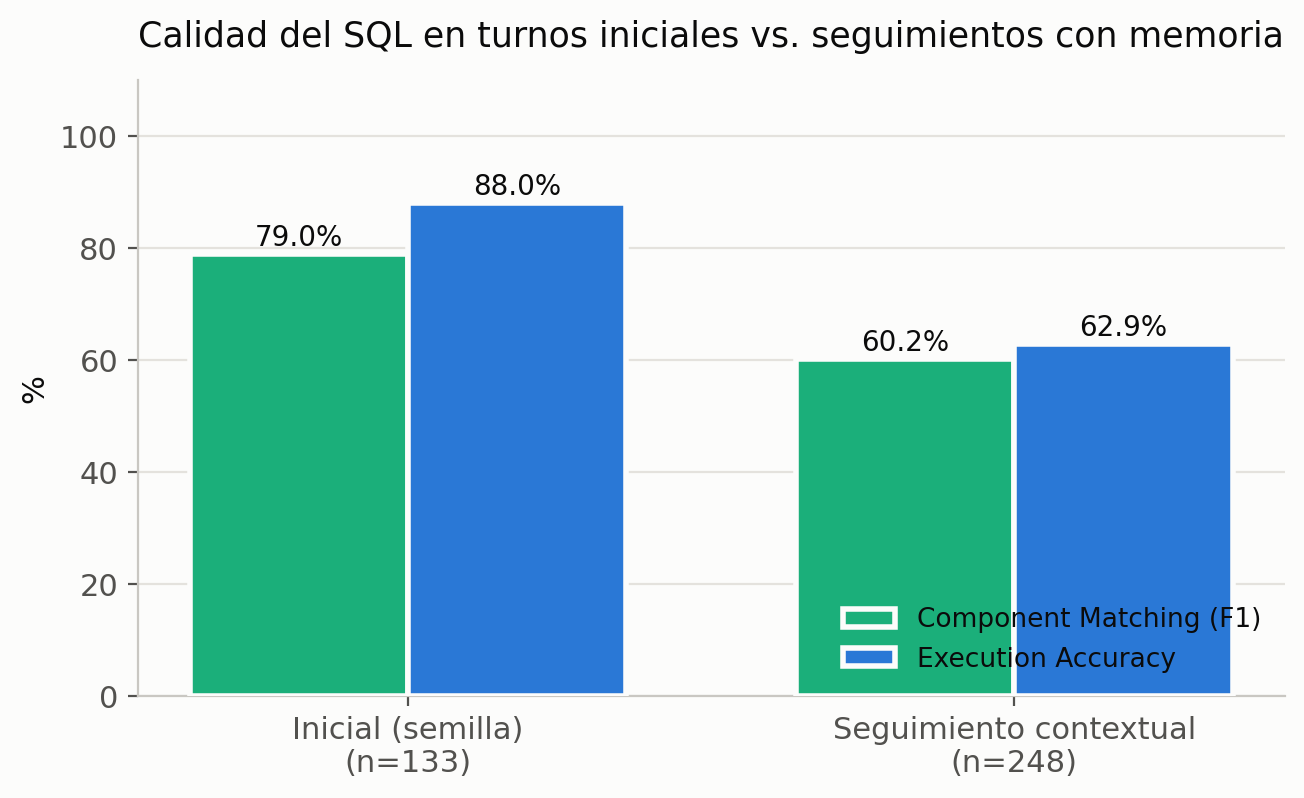
\includegraphics[width=0.63\linewidth]{Figura 5.11 - Contexto multiturno.png}
	\caption{Calidad del SQL en turnos iniciales frente a seguimientos que dependen de la memoria conversacional. La caída de Execution Accuracy (88,0\% $\rightarrow$ 62,9\%) refleja la mayor dificultad de reconstruir la consulta desde el contexto, capacidad habilitada por el módulo de Memoria.}
	\label{fig:contexto_mt}
\end{figure}

Este comportamiento se explica por la integración conjunta de los módulos de Intensión y Memoria. El módulo de Intensión evita ejecuciones prematuras cuando la información es insuficiente, mientras que el módulo de Memoria preserva representaciones del contexto previo (entidades, proyecciones y restricciones), permitiendo su reutilización controlada en turnos posteriores. En conjunto, estos mecanismos permiten que el sistema ejecute consultas únicamente cuando la información semántica necesaria ha sido correctamente inferida, mejorando la robustez y naturalidad de la interacción.

En síntesis, la evaluación conversacional evidencia que la configuración completa \textbf{RAG+Memoria+Intensión+DIN+DEA} es la única que soporta de forma consistente las interacciones multi-turno: aunque en un solo turno no maximiza la Execution Accuracy, es la que integra los componentes (Memoria e Intensión) que habilitan tanto el \emph{gating} correcto de la ejecución como la resolución de contexto, requisitos fundamentales para el despliegue de sistemas Text-to-SQL en entornos ERP conversacionales reales.

\subsection{Medición del Task Success Rate (TSR)}

El Task Success Rate (TSR) mide la capacidad del sistema para seleccionar y ejecutar la acción final correcta en cada turno, de acuerdo con la intención del usuario. A diferencia de métricas centradas únicamente en la calidad del SQL (p. ej., Execution Accuracy), el TSR evalúa el comportamiento del sistema end-to-end, incorporando tanto solicitudes ejecutables (que deben traducirse a SQL) como interacciones conversacionales (que no deben disparar ejecución).

En el sistema propuesto se definen dos acciones finales posibles:

\begin{itemize}
	\item \textbf{Conversación natural:} el sistema responde de forma informativa o aclaratoria sin generar ni ejecutar SQL.
	\item \textbf{Generar y ejecutar SQL:} el sistema traduce la solicitud del usuario a una consulta SQL y la ejecuta sobre la base de datos.
\end{itemize}

Un turno se considera exitoso (TSR\_hit) cuando la acción realizada por el sistema coincide con la acción esperada según la intención del usuario. En particular, el sistema debe evitar ejecuciones prematuras cuando la entrada es ambigua, insuficiente o puramente conversacional, y debe generar/ejecutar SQL únicamente cuando la información semántica necesaria ha sido determinada (ya sea explícitamente o mediante memoria contextual).

En el diálogo ilustrativo de once turnos del escenario base (Sección~\ref{sec:crr_dialogo}), el sistema seleccionó correctamente la acción en todos los casos, para un TSR de $11/11 = 100\%$. Para obtener una medida representativa más allá de un único diálogo, el TSR se evaluó sobre el conjunto conversacional completo.

\subsubsection{Resultados sobre el conjunto conversacional completo}

Con el fin de obtener una medida estadísticamente representativa —y no limitada a un único diálogo—, el TSR se evaluó sobre el conjunto conversacional multi-turno completo descrito en la Sección~\ref{sec:datasets}, ejecutando el flujo agentivo completo contra la base de datos de prueba. Sobre los \textbf{759 turnos} de las \textbf{100 conversaciones}, el sistema alcanzó un \textbf{TSR del 98,4\%} (747/759). El desglose por tipo de turno es revelador (Figura~\ref{fig:gating_mt}):

\begin{itemize}
	\item En los \textbf{446 turnos que debían ejecutar SQL}, el sistema ejecutó SQL en el 98,2\% de los casos (438/446): casi nunca se abstuvo indebidamente.
	\item En los \textbf{196 turnos puramente conversacionales} (saludos, cortesías, preguntas fuera de dominio), el sistema respondió sin ejecutar SQL en el 100\% de los casos: nunca disparó una consulta innecesaria.
	\item En los \textbf{117 turnos ambiguos}, el sistema solicitó aclaración en el 96,6\% de los casos (113/117); los turnos restantes constituyen el margen de error, donde intentó responder pese a la ambigüedad.
\end{itemize}

\begin{figure}[htbp]
	\centering
	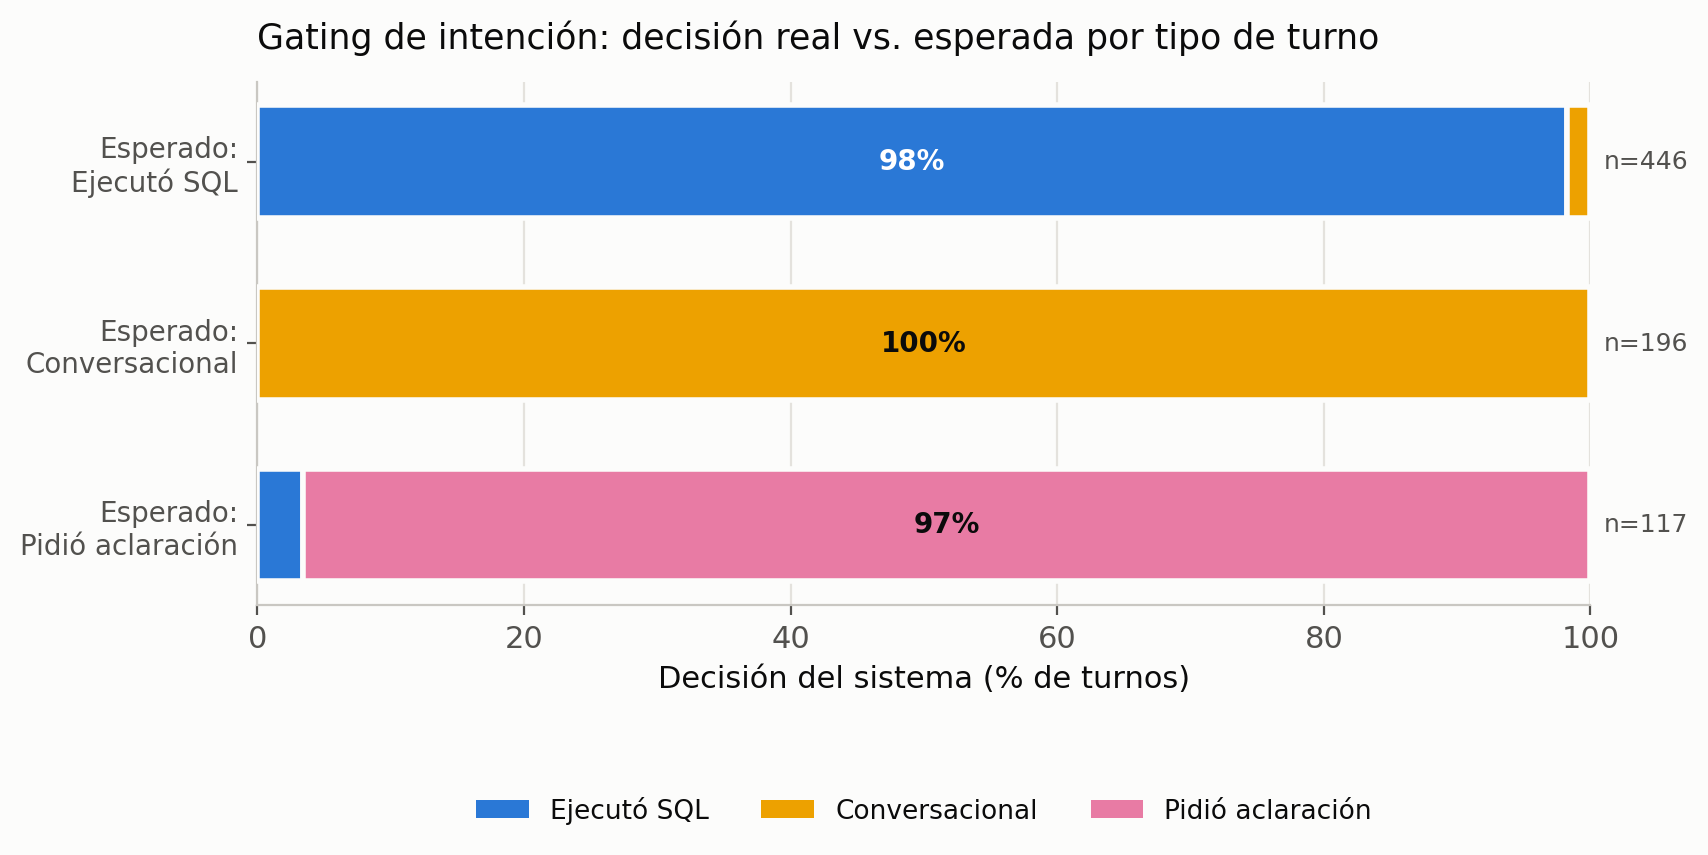
\includegraphics[width=0.76\linewidth]{Figura 5.10 - Gating multiturno.png}
	\caption{Gating de intención en el conjunto conversacional (100 conversaciones, 759 turnos): decisión real del sistema frente a la acción esperada, por tipo de turno. El sistema ejecuta SQL cuando corresponde (98,2\% en turnos ejecutables, 100\% en conversacionales), y el margen de error se concentra en los turnos ambiguos.}
	\label{fig:gating_mt}
\end{figure}

Este resultado confirma, ahora a escala del conjunto completo, que el componente de Intensión distingue de forma consistente entre (i) solicitudes conversacionales, que requieren respuesta natural sin ejecución, y (ii) solicitudes ejecutables, que deben traducirse y ejecutarse como SQL.

Este comportamiento es especialmente relevante en escenarios multi-turno, donde el sistema debe decidir si una solicitud puede resolverse mediante el uso de memoria contextual (p. ej., ``lo mismo'', ``ahora con\ldots'') o si debe solicitar aclaraciones adicionales antes de proceder. En este sentido, el TSR complementa métricas como Execution Accuracy, Context Retention Rate (CRR) y Time-to-Answer (TTA), al aportar una medida global del correcto funcionamiento del sistema desde la perspectiva del usuario final.

Finalmente, es importante destacar que un TSR del 100\% no implica que el sistema siempre genere el SQL perfecto en el primer intento; implica que el sistema toma consistentemente la decisión correcta sobre si debe o no ejecutar una consulta. En entornos productivos, esta propiedad es crítica: ejecutar SQL cuando no corresponde puede producir resultados irrelevantes o inconsistentes, incluso si la consulta es sintácticamente válida. Por tanto, el TSR obtenido sugiere que la arquitectura propuesta alcanza un control robusto del flujo de ejecución, condición necesaria para su uso en sistemas ERP donde la precisión semántica y la seguridad operativa son prioritarias.

\section{Conclusiones}

Los resultados del estudio evidencian que los módulos de razonamiento estructural, particularmente DIN y DEA, son necesarios para incrementar la Execution Accuracy en el problema Text-to-SQL. Sin embargo, su efectividad depende de manera crítica de la incorporación de mecanismos de grounding contextual. En ausencia de recuperación de contexto externo, incluso configuraciones con alto alineamiento estructural presentan tasas elevadas de error en ejecución, especialmente en esquemas extensos y con múltiples relaciones implícitas. En consecuencia, se confirma la necesidad de integrar conocimiento contextual explícito durante la generación de consultas SQL en dominios empresariales.

El componente de Intensión presenta un rol funcionalmente distinto al razonamiento estructural. Su propósito no se orienta a optimizar la forma de la consulta generada, sino a determinar si la entrada del usuario contiene información semántica suficiente para su ejecución como SQL. Este mecanismo reduce ejecuciones prematuras ante solicitudes incompletas, ambiguas o conversacionales y regula el flujo de ejecución del sistema. Este comportamiento se refleja en un Task Success Rate (TSR) del 98,4 % sobre las 100 conversaciones evaluadas (759 turnos), con un desempeño casi perfecto en los turnos que deben ejecutar SQL (98,2 %), perfecto en los puramente conversacionales (100 %), y un margen de error concentrado en los turnos ambiguos. Esto sugiere que, en contextos conversacionales, la utilidad práctica del sistema depende tanto de la exactitud de ejecución como de su capacidad para decidir cuándo abstenerse de ejecutar.

De manera complementaria, el módulo de Memoria contribuye a la coherencia contextual en escenarios multi-turno, donde la información requerida para la consulta se distribuye a lo largo de varios mensajes. La combinación de Intensión y Memoria permite reconstruir consultas completas a partir de referencias elípticas o anafóricas, sin exigir que el usuario formule una solicitud completa en un único turno. En la evaluación conversacional, el sistema reconoció y actuó sobre el contexto en el 97,4 % de los turnos de seguimiento dependientes de memoria, alcanzando una Execution Accuracy del 62,9 % en dichos turnos frente al 88,0 % de los turnos iniciales; esta brecha refleja la mayor dificultad de reconstruir la consulta desde el diálogo, y confirma que la configuración completa RAG+Memoria+Intensión+DIN+DEA —pese a no maximizar la exactitud de un solo turno— es la más adecuada para el escenario conversacional real, al ser la única que habilita simultáneamente el gating de intención y la resolución de contexto.

El análisis del Time-to-Answer (TTA) indica que un mayor tiempo de respuesta no implica necesariamente un razonamiento más efectivo. Por el contrario, configuraciones con bajo desempeño en generación inicial tienden a incrementar el TTA debido a ciclos repetidos de ejecución y corrección. En consecuencia, la eficiencia temporal del sistema se encuentra condicionada principalmente por su capacidad de generar consultas correctas desde el primer intento, más que por la complejidad del razonamiento aplicado.

Asimismo, se observa que métricas de robustez como SIN ERRORES pueden sobreestimar la capacidad real del sistema cuando existen mecanismos de autocorrección. En este sentido, la métrica SIN\_AUTO\_CORRECCION ofrece una evaluación más estricta al cuantificar la proporción de consultas correctas generadas desde el primer intento, sin dependencia de ciclos posteriores de ajuste. Esta distinción resulta relevante para la evaluación del desempeño en escenarios de uso real, donde los errores iniciales impactan la experiencia del usuario y el consumo de recursos.

Adicionalmente, los resultados resaltan el impacto del diseño del esquema de datos en el desempeño de sistemas Text-to-SQL. La base de datos de Fail Fast, al haber sido diseñada con estructura coherente, documentación y nomenclaturas alineadas con el significado funcional de tablas y columnas, reduce ambigüedades semánticas y favorece el schema linking. En consecuencia, los resultados obtenidos reflejan tanto el aporte de la arquitectura propuesta como la influencia de un diseño de datos consistente con principios semánticos claros.

Desde una perspectiva de ingeniería del sistema, la observabilidad emerge como un componente operativo necesario en arquitecturas multi-agente. El uso de plataformas low-code como n8n permitió orquestar el flujo agentivo como una secuencia explícita de componentes trazables, posibilitando inspección por etapa de entradas, decisiones intermedias, contexto utilizado, SQL propuesto, errores y correcciones. Esta trazabilidad facilita la identificación sistemática de patrones de falla, el análisis comparativo entre configuraciones y la reutilización de peticiones fallidas como insumo para iteraciones de mejora y priorización de ajustes mediante estudios de ablación.

Finalmente, la configuración [RAG + DIN + DEA] se establece como la alternativa más balanceada para generación directa de SQL, al presentar el mejor compromiso entre simplicidad, exactitud de ejecución y confiabilidad. No obstante, en escenarios conversacionales, la integración de Intensión y Memoria resulta necesaria para asegurar que la ejecución se realice únicamente cuando la consulta sea semánticamente válida y contextualmente completa. En conjunto, los resultados apoyan la hipótesis de que una arquitectura híbrida modular y multi-agente mejora la precisión y la robustez del proceso Text-to-SQL en un ERP real, y sugieren que estos sistemas deben concebirse como workflows cognitivos observables y auditables, en lugar de traductores monolíticos de lenguaje natural a SQL.

\section{Trabajo Futuro}

Si bien los resultados obtenidos son alentadores, este trabajo abre múltiples líneas de investigación y desarrollo futuro. En primer lugar, la arquitectura propuesta podría ampliarse incorporando mecanismos predictivos, orientados a anticipar la intención del usuario o a sugerir consultas relevantes basadas en patrones históricos de interacción. Este enfoque permitiría reducir aún más el tiempo de respuesta y mejorar la experiencia del usuario en escenarios exploratorios o recurrentes.

En segundo lugar, una extensión natural del sistema consiste en avanzar hacia interacciones multimodales, donde las consultas no se originen únicamente a partir de texto, sino también desde otros tipos de entrada como imágenes, tablas, documentos o interfaces visuales. Por ejemplo, permitir que un usuario seleccione visualmente un elemento de un reporte o una imagen de inventario y formule una pregunta contextualizada podría ampliar significativamente las capacidades del sistema más allá del paradigma Text-to-SQL tradicional.

Adicionalmente, futuras investigaciones podrían explorar la integración de GraphRAG \cite{han2025graphrag} u otros mecanismos de recuperación estructurada que modelen explícitamente relaciones complejas entre entidades del ERP, con el fin de mejorar el razonamiento en consultas que requieran múltiples saltos lógicos o dependencias implícitas entre tablas.

Otra línea relevante de trabajo futuro consiste en evaluar el sistema en entornos productivos de mayor escala, considerando esquemas con cientos o miles de tablas, múltiples compañías (multi-tenant) y reglas de negocio más complejas. Esto permitiría analizar aspectos como escalabilidad, costos computacionales y comportamiento bajo cargas reales de usuarios.

Finalmente, se abre la posibilidad de incorporar agentes especializados adicionales, orientados a validación semántica, explicación de resultados o control de seguridad y permisos, reforzando la trazabilidad y gobernanza del sistema. Estas extensiones permitirían evolucionar el ERP hacia una interfaz cognitiva más completa, donde la consulta, el análisis y la explicación de la información empresarial se integren de forma natural, segura y escalable.

\appendix

\section{Conjunto de consultas de evaluación Text-to-SQL en el ERP Fail Fast}

\subsection{Descripción general del conjunto de consultas}

Este anexo presenta el conjunto de consultas de referencia (\textit{gold queries}) utilizado para la evaluación del sistema Text-to-SQL propuesto. Dicho conjunto fue construido manualmente a partir de escenarios reales de uso del ERP Fail Fast, con el objetivo de reflejar preguntas típicas formuladas por usuarios empresariales sin conocimientos técnicos en SQL.

Cada consulta documentada en este anexo incluye:

\begin{itemize}
	\item La formulación original de la pregunta en lenguaje natural.
	\item La clasificación por nivel de complejidad (baja, media o alta).
	\item La descomposición semántica empleada para su resolución.
	\item La identificación de las tablas y columnas relevantes del esquema.
	\item La consulta SQL de referencia (\textit{gold standard}), validada contra la base de datos real del sistema.
\end{itemize}

Este nivel de detalle permite asegurar trazabilidad metodológica, facilitar la reproducibilidad del experimento y habilitar análisis posteriores sobre patrones de error y comportamiento del sistema.

\subsection{Consultas de complejidad baja}

Las consultas de complejidad baja se caracterizan por involucrar una única tabla o un conjunto reducido de columnas, con filtros directos y, en algunos casos, operaciones simples de ordenamiento o conteo. Este tipo de consultas representa solicitudes frecuentes de tipo informativo, como la obtención de registros recientes, conteos básicos o la recuperación de atributos específicos de una entidad.

Su inclusión permite evaluar la capacidad del sistema para manejar correctamente escenarios elementales sin introducir errores innecesarios en la selección de tablas, columnas o condiciones de filtrado.

\begin{figure}[htbp]
	\centering
	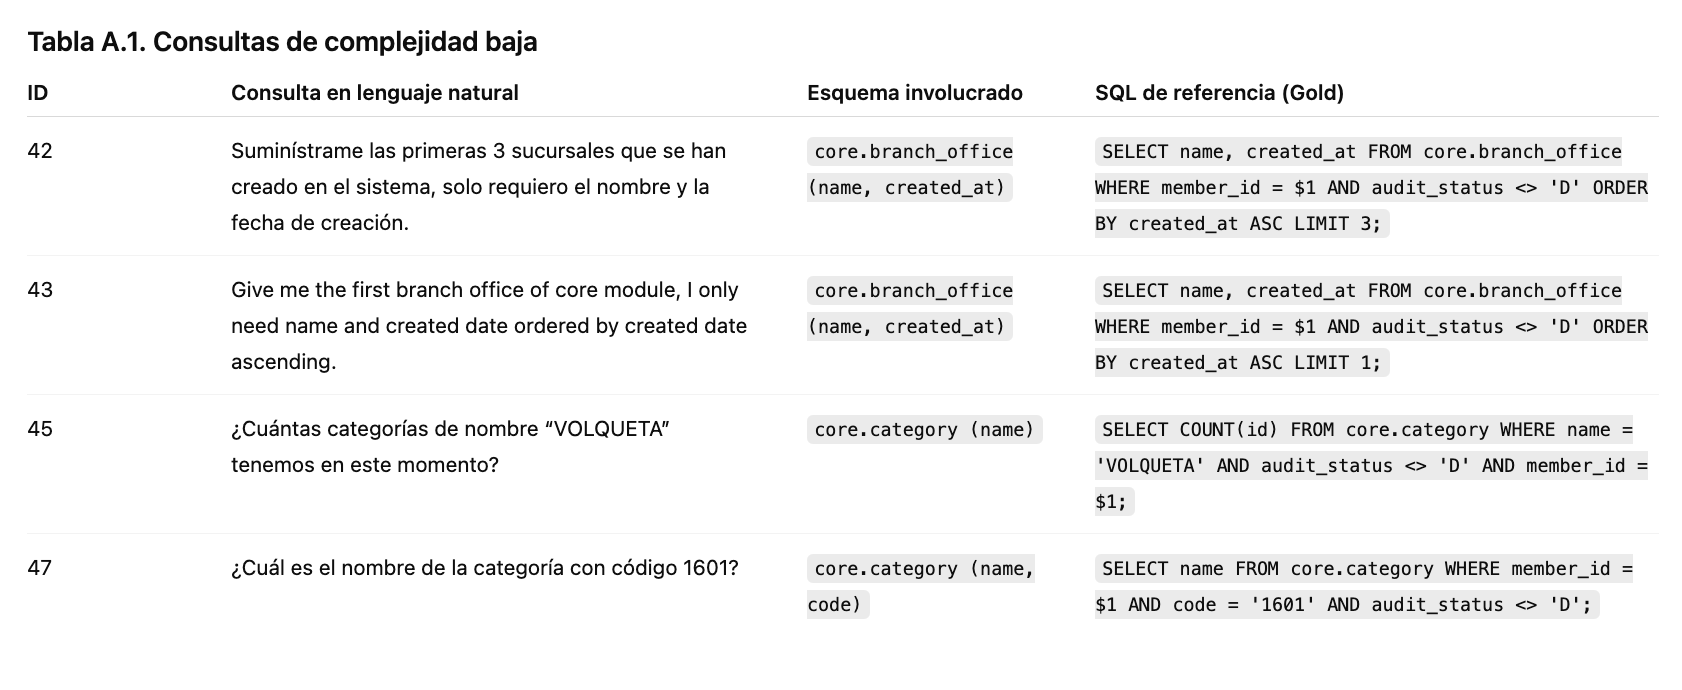
\includegraphics[width=0.88\linewidth]{Tabla 1.png}
	\caption{Consultas de complejidad baja utilizadas en la evaluación}
	\label{fig:anexo_baja}
\end{figure}

\subsection{Consultas de complejidad media}

Las consultas de complejidad media involucran operaciones de agregación (\texttt{SUM}, \texttt{COUNT}), cláusulas de agrupamiento (\texttt{GROUP BY}) y, en algunos casos, combinaciones simples entre tablas. Estas consultas requieren una identificación explícita de la clave de agrupación y la correcta aplicación del contexto multi-tenant del sistema.

Este nivel de complejidad es representativo de reportes operativos y financieros comunes en sistemas ERP reales.

\begin{figure}[htbp]
	\centering
	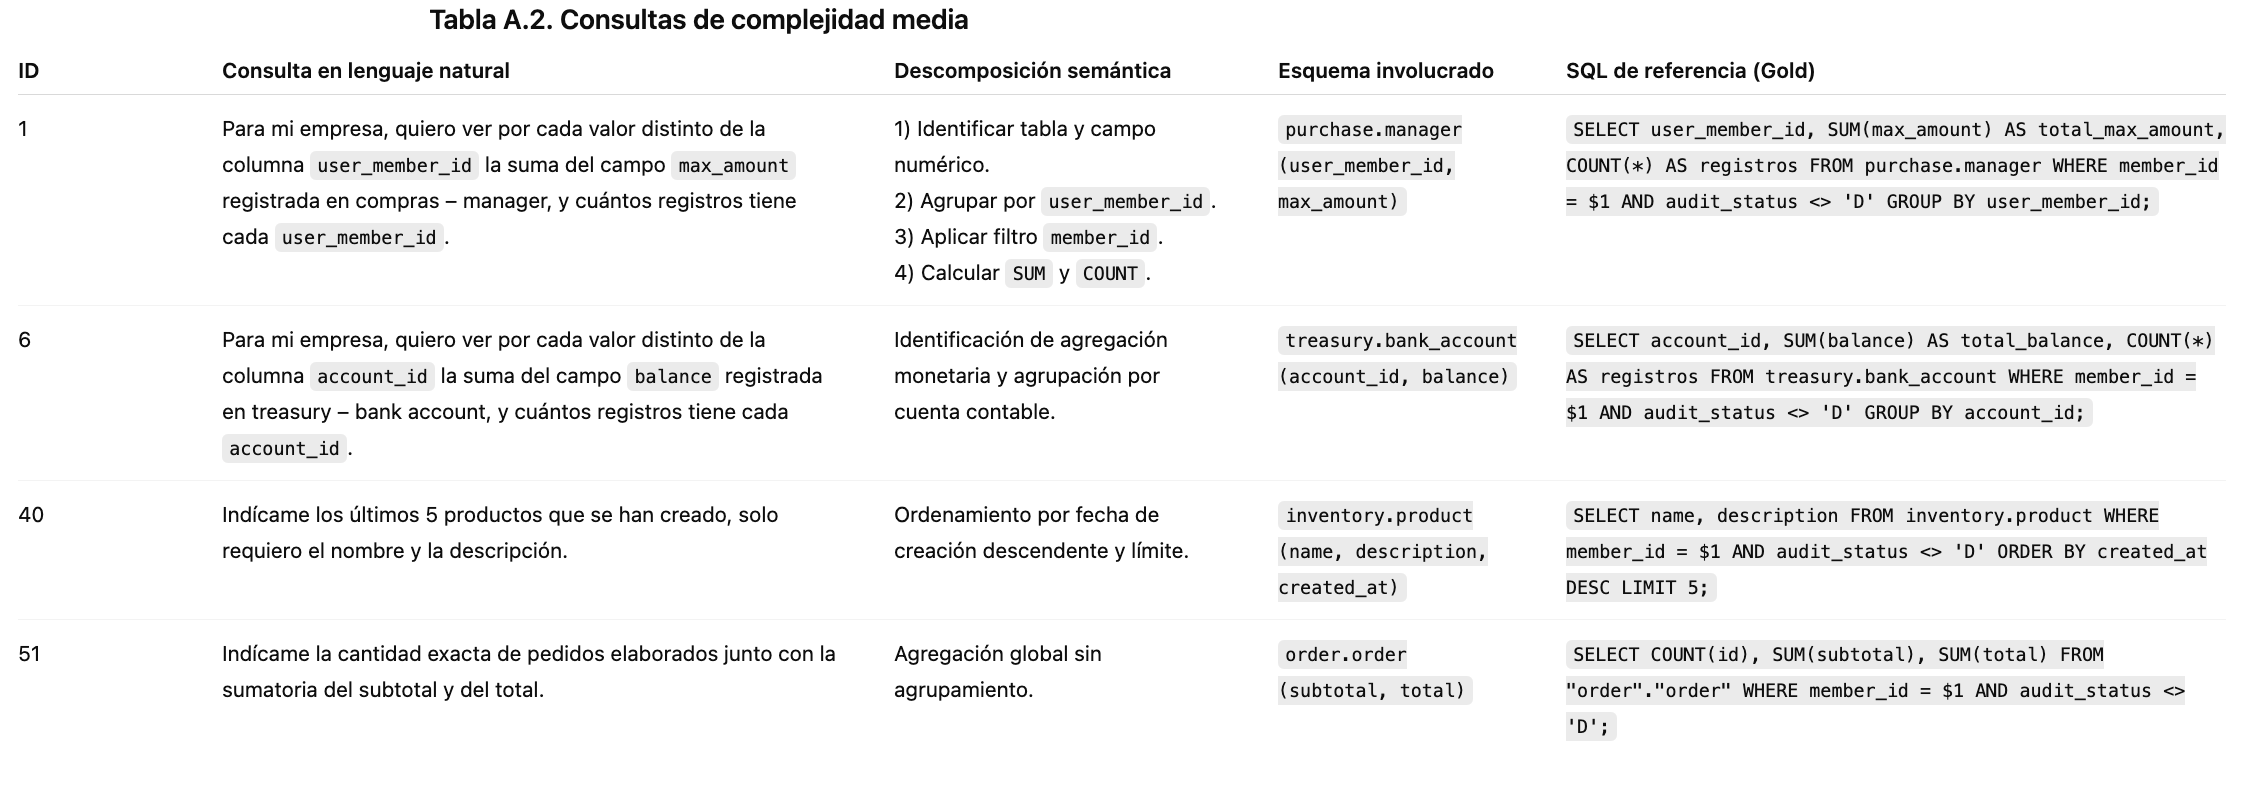
\includegraphics[width=0.88\linewidth]{Tabla 2.png}
	\caption{Consultas de complejidad media utilizadas en la evaluación}
	\label{fig:anexo_media}
\end{figure}

\subsection{Consultas de complejidad alta}

Las consultas de complejidad alta requieren combinaciones entre múltiples tablas pertenecientes a distintos módulos del ERP, así como razonamiento multietapa para integrar información distribuida en el esquema. En estos casos, la resolución de la consulta implica descomponer la pregunta original en sub-tareas, resolver dependencias entre entidades y aplicar agregaciones sobre los resultados combinados.

\begin{figure}[htbp]
	\centering
	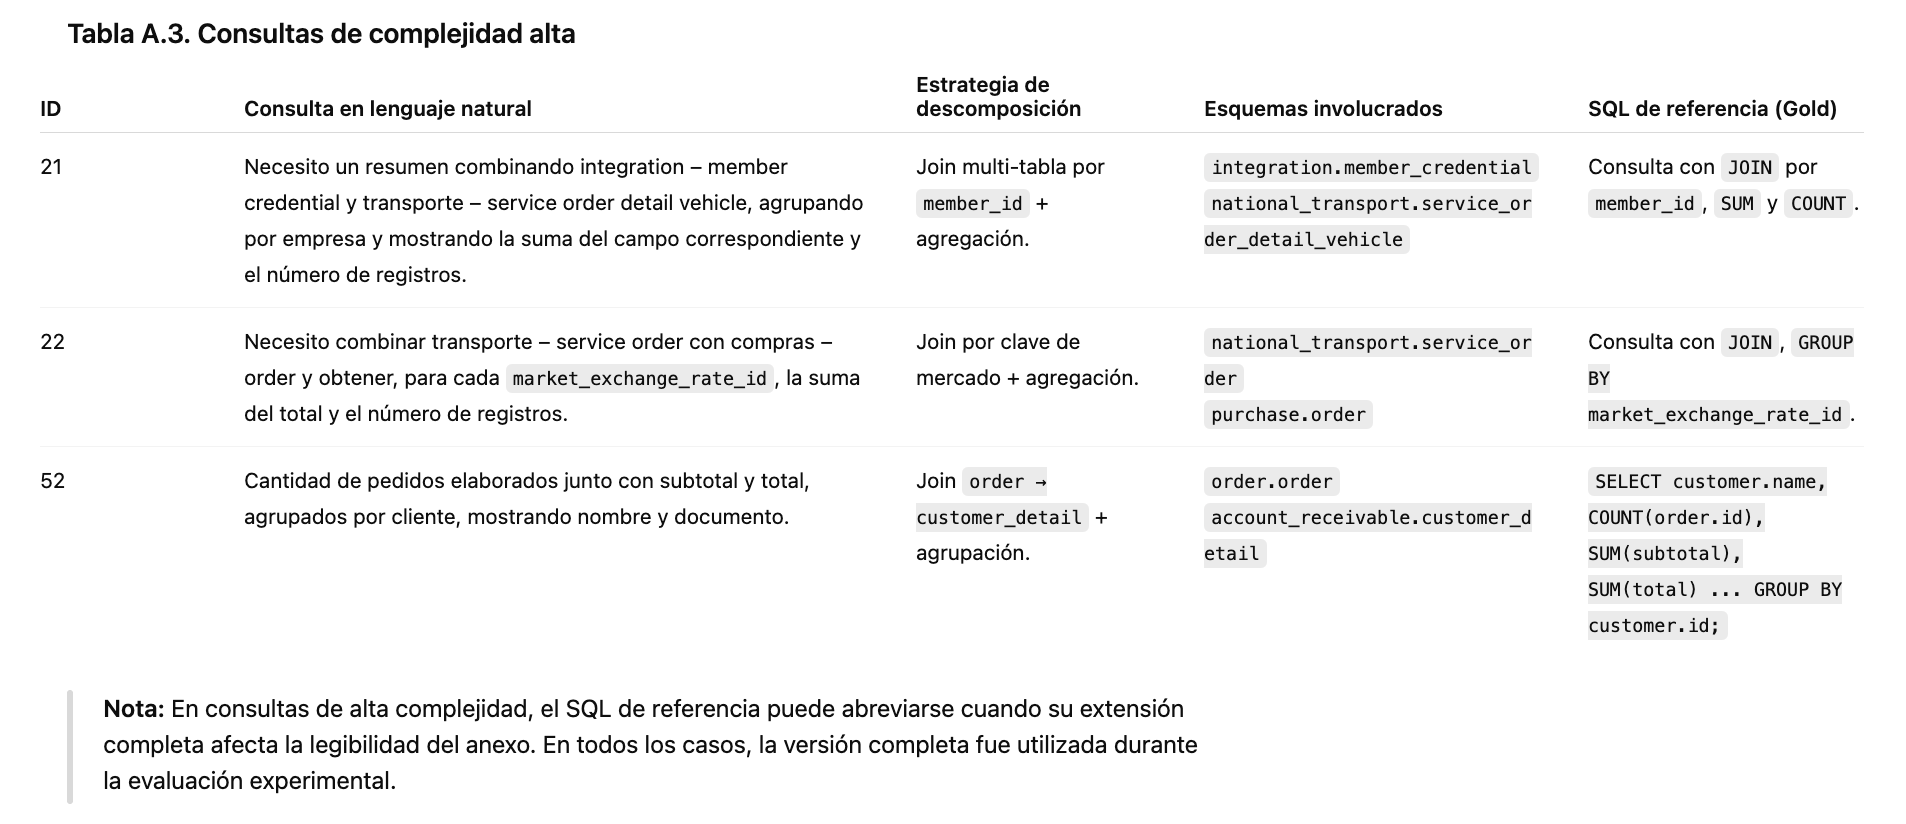
\includegraphics[width=0.88\linewidth]{Tabla 3.png}
	\caption{Consultas de complejidad alta utilizadas en la evaluación}
	\label{fig:anexo_alta}
\end{figure}

\textbf{Nota:} En las consultas de mayor complejidad, el SQL de referencia puede presentarse de forma abreviada cuando su extensión completa afecta la legibilidad del anexo. En todos los casos, la versión completa fue utilizada durante la evaluación experimental.

\subsection{Observaciones metodológicas}

Las consultas incluidas en este anexo fueron diseñadas para cubrir patrones frecuentes de interacción en sistemas ERP reales, tales como agregaciones financieras, consultas multi-tabla, análisis temporal y reportes operativos. Su documentación detallada permite complementar la metodología experimental descrita en el Capítulo IV y facilitar la replicación del estudio.

\begin{thebibliography}{99}

	\bibitem{yu2018spider}
	T. Yu et al., ``Spider: A large-scale human-labeled dataset for complex and cross-domain semantic parsing and text-to-SQL task,'' in \textit{Proc. EMNLP}, Brussels, Belgium, 2018, pp. 3911--3921.

	\bibitem{scholak2021picard}
	T. Scholak, N. Schucher, and D. Bahdanau, ``PICARD: Parsing incrementally for constrained auto-regressive decoding from language models,'' in \textit{Proc. EMNLP}, Punta Cana, Dominican Republic, 2021, pp. 9895--9901.

	\bibitem{pourreza2023din}
	M. Pourreza and D. Rafiei, ``DIN-SQL: Decomposed in-context learning of text-to-SQL with self-correction,'' in \textit{Proc. NeurIPS}, New Orleans, LA, USA, 2023.

	\bibitem{gan2021natural}
	Y. Gan, X. Chen, and M. Purver, ``Exploring underexplored limitations of cross-domain text-to-SQL generalization,'' in \textit{Proc. EMNLP}, Punta Cana, Dominican Republic, 2021, pp. 8926--8931.

	\bibitem{hong2024bird}
	J. Li et al., ``Can LLM already serve as a database interface? A BIg bench for large-scale database grounded text-to-SQLs,'' in \textit{Proc. NeurIPS Datasets and Benchmarks Track}, New Orleans, LA, USA, 2023.

	\bibitem{shi2025comprehensive}
	L. Shi et al., ``A survey on employing large language models for text-to-SQL tasks,'' \textit{ACM Comput. Surv.}, vol. 58, no. 2, pp. 1--37, 2025, doi: 10.1145/3737873.

	\bibitem{liu2025survey}
	X. Liu et al., ``A survey of text-to-SQL in the era of LLMs: Where are we, and where are we going?,'' \textit{IEEE Trans. Knowl. Data Eng.}, vol. 37, no. 10, pp. 5735--5754, 2025, doi: 10.1109/TKDE.2025.3592032.

	\bibitem{hong2025advances}
	Z. Hong et al., ``Next-generation database interfaces: A survey of LLM-based text-to-SQL,'' \textit{IEEE Trans. Knowl. Data Eng.}, vol. 37, no. 12, pp. 7328--7345, Dec. 2025, doi: 10.1109/TKDE.2025.3609486.

	\bibitem{li2014nalir}
	F. Li and H. V. Jagadish, ``Constructing an interactive natural language interface for relational databases,'' \textit{Proc. VLDB Endow.}, vol. 8, no. 1, pp. 73--84, Sep. 2014.

	\bibitem{yaghmazadeh2017sqlizer}
	Y. Yaghmazadeh et al., ``SQLizer: Query synthesis from natural language,'' \textit{Proc. ACM Program. Lang.}, vol. 1, no. OOPSLA, pp. 63:1--63:26, Oct. 2017.

	\bibitem{dong2016language}
	L. Dong and M. Lapata, ``Language to logical form with neural attention,'' in \textit{Proc. ACL (Volume 1: Long Papers)}, Berlin, Germany, 2016, pp. 33--43.

	\bibitem{li2023resdsql}
	H. Li et al., ``RESDSQL: Decoupling schema linking and skeleton parsing for text-to-SQL,'' in \textit{Proc. AAAI}, vol. 37, no. 11, Washington, DC, USA, 2023, pp. 13067--13075, doi: 10.1609/aaai.v37i11.26535.

	\bibitem{huang2024survey}
	Y. Huang et al., ``Exploring the landscape of text-to-SQL with large language models: Progresses, challenges and opportunities,'' arXiv preprint arXiv:2505.23838, 2025.

	\bibitem{xie2024dea}
	Y. Xie et al., ``Decomposition for enhancing attention: Improving LLM-based text-to-SQL through workflow paradigm (DEA-SQL),'' in \textit{Findings of ACL}, Bangkok, Thailand, 2024, pp. 10796--10816.

	\bibitem{li2024comprehensive}
	B. Zhang et al., ``SQLBench: A comprehensive evaluation for text-to-SQL capabilities of large language models,'' arXiv preprint arXiv:2403.02951, 2024.

	\bibitem{wang2025mac}
	B. Wang et al., ``MAC-SQL: A multi-agent collaborative framework for text-to-SQL,'' in \textit{Proc. COLING}, Abu Dhabi, UAE, 2025, pp. 540--557.

	\bibitem{li2024codes}
	H. Li et al., ``CodeS: Towards building open-source language models for text-to-SQL,'' \textit{Proc. ACM Manag. Data}, vol. 2, no. 3, art. 127, 2024, doi: 10.1145/3654930.

	\bibitem{han2025graphrag}
	H. Han et al., ``Retrieval-augmented generation with graphs (GraphRAG),'' arXiv preprint arXiv:2501.00309, 2025.

	\bibitem{aparicio2023natural}
	S. Aparicio et al., ``Natural language to SQL in low-code platforms,'' arXiv preprint arXiv:2308.15239, 2023.

	\bibitem{dou2022towards}
	L. Dou et al., ``Towards knowledge-intensive text-to-SQL semantic parsing with formulaic knowledge,'' in \textit{Proc. EMNLP}, Abu Dhabi, UAE, 2022, pp. 5240--5253.

	\bibitem{hong2024knowledge}
	Z. Hong et al., ``Knowledge-to-SQL: Enhancing SQL generation with data expert LLM,'' in \textit{Findings of ACL}, Bangkok, Thailand, 2024, pp. 10997--11008, doi: 10.18653/v1/2024.findings-acl.653.

	\bibitem{gao2024dail}
	D. Gao et al., ``Text-to-SQL empowered by large language models: A benchmark evaluation (DAIL-SQL),'' \textit{Proc. VLDB Endow.}, vol. 17, no. 5, pp. 1132--1145, 2024, doi: 10.14778/3641204.3641221.

	\bibitem{lee2024mcs}
	D. Lee et al., ``MCS-SQL: Leveraging multiple prompts and multiple-choice selection for text-to-SQL generation,'' in \textit{Proc. COLING}, Abu Dhabi, UAE, 2025, pp. 337--353.

	\bibitem{talaei2024chess}
	S. Talaei et al., ``CHESS: Contextual harnessing for efficient SQL synthesis,'' arXiv preprint arXiv:2405.16755, 2024.

	\bibitem{zhang2023act}
	H. Zhang et al., ``ACT-SQL: In-context learning for text-to-SQL with automatically-generated chain-of-thought,'' in \textit{Findings of EMNLP}, Singapore, 2023, pp. 3501--3532.

	\bibitem{rai2023improving}
	D. Rai et al., ``Improving generalization in language model-based text-to-SQL semantic parsing: Two simple semantic boundary-based techniques,'' in \textit{Proc. ACL (Volume 2: Short Papers)}, Toronto, Canada, 2023, pp. 150--160.

	\bibitem{singh2025survey}
	A. Singh et al., ``A survey of large language model-based generative AI for text-to-SQL: Benchmarks, applications, use cases, and challenges,'' arXiv preprint arXiv:2412.05208, 2024.

	\bibitem{zhu2024large}
	X. Zhu et al., ``Large language model enhanced text-to-SQL generation: A survey,'' arXiv preprint arXiv:2410.06011, 2024.

\end{thebibliography}

\end{document}
